%% This is file `DEMO-TUDaThesis.tex' version 3.07 (2020/10/21),
%% it is part of
%% TUDa-CI -- Corporate Design for TU Darmstadt
%% ----------------------------------------------------------------------------
%%
%%  Copyright (C) 2018--2020 by Marei Peischl <marei@peitex.de>
%%
%% ============================================================================
%% This work may be distributed and/or modified under the
%% conditions of the LaTeX Project Public License, either version 1.3c
%% of this license or (at your option) any later version.
%% The latest version of this license is in
%% http://www.latex-project.org/lppl.txt
%% and version 1.3c or later is part of all distributions of LaTeX
%% version 2008/05/04 or later.
%%
%% This work has the LPPL maintenance status `maintained'.
%%
%% The Current Maintainers of this work are
%%   Marei Peischl <tuda-ci@peitex.de>
%%   Markus Lazanowski <latex@ce.tu-darmstadt.de>
%%
%% The development respository can be found at
%% https://github.com/tudace/tuda_latex_templates
%% Please use the issue tracker for feedback!
%%
%% If you need a compiled version of this document, have a look at
%% http://mirror.ctan.org/tex-archive/macros/latex/contrib/tuda-ci/doc
%% or at the documentation directory of this package (if installed)
%% <path to your LaTeX distribution>/doc/latex/tuda-ci
%% ============================================================================
%%
% !TeX program = lualatex
%%

\documentclass[
	%ngerman,
	ruledheaders=section,%Ebene bis zu der die Überschriften mit Linien abgetrennt werden, vgl. DEMO-TUDaPub
	class=report,% Basisdokumentenklasse. Wählt die Korrespondierende KOMA-Script Klasse
	thesis={type=master},% Dokumententyp Thesis, für Dissertationen siehe die Demo-Datei DEMO-TUDaPhd
	accentcolor=9c,% Auswahl der Akzentfarbe
	% custommargins=true,% Ränder werden mithilfe von typearea automatisch berechnet
	marginpar=false,% Kopfzeile und Fußzeile erstrecken sich nicht über die Randnotizspalte
	%BCOR=5mm,%Bindekorrektur, falls notwendig
	parskip=half-,%Absatzkennzeichnung durch Abstand vgl. KOMA-Sript
	fontsize=11pt,%Basisschriftgröße laut Corporate Design ist mit 9pt häufig zu klein
	logofile=img/tuda_logo, %Falls die Logo Dateien nicht vorliegen
]{tudapub}


% Der folgende Block ist nur bei pdfTeX auf Versionen vor April 2018 notwendig
\usepackage{iftex}
\ifPDFTeX
	\usepackage[utf8]{inputenc}%kompatibilität mit TeX Versionen vor April 2018
\fi

%%%%%%%%%%%%%%%%%%%
%Sprachanpassung & Verbesserte Trennregeln
%%%%%%%%%%%%%%%%%%%
\usepackage[ngerman, main=english]{babel}
\usepackage[autostyle]{csquotes}% Anführungszeichen vereinfacht

% Falls mit pdflatex kompiliert wird, wird microtype automatisch geladen, in diesem Fall muss diese Zeile entfernt werden, und falls weiter Optionen hinzugefügt werden sollen, muss dies über
% \PassOptionsToPackage{Optionen}{microtype}
% vor \documentclass hinzugefügt werden.
\usepackage{microtype}

%%%%%%%%%%%%%%%%%%%
%Literaturverzeichnis
%%%%%%%%%%%%%%%%%%%
\usepackage{biblatex}   % Literaturverzeichnis

%%%%%%%%%%%%%%%%%%%
%Abkürzungsverzeichnis
%%%%%%%%%%%%%%%%%%%
\usepackage[printonlyused]{acronym}

\usepackage{cleveref}

%%%%%%%%%%%%%%%%%%%
%Paketvorschläge Tabellen
%%%%%%%%%%%%%%%%%%%
%\usepackage{array}     % Basispaket für Tabellenkonfiguration, wird von den folgenden automatisch geladen
\usepackage{tabularx}   % Tabellen, die sich automatisch der Breite anpassen
%\usepackage{longtable} % Mehrseitige Tabellen
%\usepackage{xltabular} % Mehrseitige Tabellen mit anpassarer Breite
\usepackage{booktabs}   % Verbesserte Möglichkeiten für Tabellenlayout über horizontale Linien

%%%%%%%%%%%%%%%%%%%
%Paketvorschläge Mathematik
%%%%%%%%%%%%%%%%%%%
%\usepackage{mathtools} % erweiterte Fassung von amsmath
%\usepackage{amssymb}   % erweiterter Zeichensatz
%\usepackage{siunitx}   % Einheiten

% Diagrams
\usepackage{tikz}
\usetikzlibrary{shapes.geometric, arrows}

% Code
\usepackage{listings}
\lstset{basicstyle=\ttfamily,breaklines=true}

% Zapf-Dingbats Symbole
\usepackage{pifont}

% TODO Notizen
\usepackage{todonotes}
%\usepackage[disable]{todonotes}
%Formatierungen für Beispiele in diesem Dokument. Im Allgemeinen nicht notwendig!
\let\file\texttt
\let\code\texttt
\let\tbs\textbackslash

% Zapf-Dingbats Symbole
\newcommand*{\FeatureTrue}{\ding{52}}
\newcommand*{\FeatureFalse}{\ding{56}}

% Remove parentheses from referenced equations in text
\creflabelformat{equation}{#2\textup{#1}#3}

\newcommand{\eg}{e.g., }
\newcommand{\ie}{i.e., }

\lstset{
    basicstyle=\ttfamily\small,
    breaklines=true,
    numbers=left,
    stepnumber=1,
    xleftmargin=2.5em,
    frame=lines,
    framexleftmargin=2.5em
}

% ILOC simplifications
\newcommand{\iloc}[1]{\texttt{\small#1}}
\newcommand{\ilocreg}[1]{\iloc{r\textsubscript{#1}}}
\newcommand{\ilocarrow}{$\Rightarrow$}
\newcommand{\iloccmd}[3]{\iloc{#1} & \iloc{#2} & \ilocarrow & \iloc{#3}}
\newcommand{\iloccmdinl}[3]{\iloc{#1}~\iloc{#2}~\ilocarrow~\iloc{#3}}

\newcommand{\aurora}{NEC SX-Aurora TSUBASA-VE}

\newcommand{\tblsection}[1]{\emph{#1}}
\newcommand{\tblitem}[1]{\hspace{0.3cm}#1}

\hyphenation{si-mul-ta-ne-ous-ly}


% Select includes
\includeonly{
    % chapters/about_this_file,
    % chapters/template_usage,
	chapters/introduction,
    chapters/background,
    chapters/related_work,
	chapters/approach,
    chapters/evaluation,
	chapters/conclusion_and_future_work
	appendices/random-scheduling-experiment
}

\addbibresource{bibliography.bib}

\begin{document}

\Metadata{
	title=Automatic Compiler Customization for Novel Hardware,
	author=Janne Wulf
}

\title{Automatic Compiler Customization for Novel Hardware}
\subtitle{Automatische Anpassung von Compilern für neuartige Hardwarearchitekturen}
\author[J. Wulf]{Janne Wulf}%optionales Argument ist die Signatur,
\birthplace{Oldenburg in Holstein}%Geburtsort, bei Dissertationen zwingend notwendig
\reviewer{Dr. rer. nat. Stefan Guthe \and  Dr. Ing. Daniel Thuerck}%Gutachter

%Diese Felder erden untereinander auf der Titelseite platziert.
%\department ist eine notwendige Angabe, siehe auch dem Abschnitt `Abweichung von den Vorgaben für die Titelseite'
\department{inf} % Das Kürzel wird automatisch ersetzt und als Studienfach gewählt, siehe Liste der Kürzel im Dokument.
\institute{Interactive Graphics Systems Group}
\group{Perceptual Graphics, Capture and Massively Parallel Computing}

\submissiondate{August 9, 2021}
\examdate{\today}

%	\tuprints{urn=1234,printid=12345,doi=10.25534/tuprints-1234}
%	\dedication{Für alle, die \TeX{} nutzen.}

\maketitle

\affidavit
% oder \affidavit[digital] falls eine rein digitale Abgabe vorgesehen ist.

\tableofcontents

\listoftodos

\todo{Check the font. The 't' looks very small}

\chapter{Über diese Datei}
Die Datei \file{DEMO-TUDaThesis.tex} ist ein Template für Abschlussarbeiten im Stil des Corporate Designs der TU Darmstadt.
Sie ist Teil des TUDa-CI-Bundles wurde vom in Teilen tuddesign-Paket von C.~v.~Loewenich und J.~Werner inspiriert.

Sie verwendet die Dokumentenklasse \file{tudapub.cls}, allerdings mit erweiterten Einstellungen. In diesem Dokument werden überwiegend die speziell auf Abschlussarbeiten ausgelegten Möglichkeiten beschrieben. Weitere Konfigurationsmöglichkeiten finden sich in der Datei \file{DEMO-TUDaPub.pdf} \cite{tudapub}.

Es ist voreingestellt, dass eine PDF/A-Datei erzeugt wird. Die beste Kompatibilität hierfür bietet Lua\LaTeX. Bei anderen Compilern kann dies entsprechend der Informationen in DEMO-TUDaPub zu Problemen führen. In diesem Fall sollte entweder der Compiler gewechselt oder \code{pdfa=false} aktiviert werden.

Für weitere Informationen kann ein Blick in die zur Dokumentenklasse gehörigen Dokumentation (tudapub.pdf) hilfreich sein. Sie wird zusammen mit den Quelldateien verteilt.

\minisec{Unterschiede der Demodateien DEMO-TUDaThesis und DEMO-TUDaPhD}
Zwar basieren alle drei DEMO-Dateien auf der Klasse \code{tudapub}, allerdings sind die Basiseinstelungen dem Dokumententyp angepasst.
Für Erläuterungen zu den TUDaPub spezifischen Optionen, sei auf die Datei DEMO-TUDaPub verwiesen.
Da die Basisklasse für beide identisch ist, kann jede Option abgeändert werden. Die Folgende Liste zeigt lediglich die gezeigten Features bei Standardeinstellungen.

\noindent\begin{tabularx}{\linewidth}{@{}p{.25\linewidth}*3{>{\centering\arraybackslash}X}@{}}
	\toprule
	Option&DEMO-TUDaThesis&DEMO-TUDaPhD&DEMO-TUDapub\\
	\midrule
	twoside&\FeatureFalse&\FeatureTrue&\FeatureFalse\\\midrule
	parskip&\FeatureTrue&\FeatureFalse&\FeatureTrue\\\midrule
	Kolophon&\FeatureFalse&\FeatureTrue&\FeatureFalse\\\midrule
	Widmung&\FeatureFalse&\FeatureTrue&\FeatureFalse\\\midrule
	Schriftgröße&11pt&11pt&9pt\\\midrule
	ruledheaders&section&chapter&all\\\midrule
	Basisklasse&scrreprt&scrbook&scrartcl\\\midrule
	thesis&\ttfamily type=bachelor&\ttfamily type=dr, dr=rernat
	&\FeatureFalse\\\midrule
	marginpar&\FeatureFalse&\FeatureFalse&\FeatureTrue\\\midrule
	Affidavit\newline\rlap{(Selbstständigkeitserklärung)}&\FeatureTrue&\FeatureTrue&\FeatureFalse\\\midrule
	abstract&\FeatureFalse&\FeatureTrue&\FeatureTrue\\\midrule
	custommargins&\FeatureTrue&\FeatureTrue&\FeatureFalse\\
	\bottomrule
\end{tabularx}

\chapter{Verwendung}
Die Klasse kann wie für Dokumentenklassen üblich eingebunden werden
\begin{verbatim}
\documentclass[thesis]{tudapub}
\end{verbatim}
Die Option \code{thesis} wechselt hierbei in den Modus, der spezielle Features für Abschlussarbeiten freischaltet, die in diesem Dokument beschrieben werden.

Darüber hinaus lässt sich die Klasse verwenden wie die Standard-KOMA-Script-Klasse, auf der sie basiert.
Voreingestellt ist hierbei \code{scrreprt}.

Allgemein bietet \KOMAScript{} viele Möglichkeiten zu Anpassungen. Wie in der tudapub-Demo-Datei beschrieben, können hier jedoch nicht alle erläutert werden, ein Blick in die offizielle Dokumentation ist daher häufig hilfreich \cite{scrguide}.

\section{Sprachanpassung}
Der Modus für Abschlussarbeiten setzt einige sprachabhängige Bezeichnungen.
Teilweise ist Deutsch für diese Elemente als Hauptsprache vorgeschrieben (z.\,B. die Selbstständigkeitserklärung). Für die korrekte Verarbeitung wird daher ein Paket zur Sprachanpassung benötigt.
TUDa-CI verwendet hierfür das babel-Paket.

Dies wird jedoch nicht automatisch geladen, da hierfür die Konfiguration der Sprachen bekannt sein müsste. Die Demo-Dateien für Abschlussarbeiten (\file{DEMO-TUDaThesis.tex}/""\file{DEMO-TUDaPhD.tex}) laden hierfür die Konfiguration:
\begin{verbatim}
	\usepackage[english, main=ngerman]{babel}
\end{verbatim}
Diese ist für ein Dokument mit Deutsch als Hauptsprache und Englischen Elementen.
Die Hauptsprache wird als Wert der Option \verb+main=+ übergeben.
Das Laden von \verb+ngerman+ wird in den Fällen, in denen es von TUDa-CI benötigt wird, automatisch ausgelöst.
Für eine bessere Übersichtlichkeit ist es dennoch hilfreich es dort aufzuführen.

Falls die Hauptsprache nicht Deutsch ist, wäre daher die folgende Konfiguration sinnvoll:
\begin{verbatim}
	\usepackage[ngerman, main=<Hauptsprache>]{babel}
\end{verbatim}

\section{Übergabe der Titelinformationen}

Die Titelinformationen werden analog zur klassichen Titelerzeugung mit \verb+\maketitle+ übergeben. Allerdings wurden die Felder um ein paar speziellere Daten erweitert. Sofern nicht anders angegeben, verfügen alle Makros über ein notwendiges Argument für die Datenübergabe, z.\,B.
\begin{verbatim}
\title{\LaTeX{} im Corporate Design der TU Darmstadt}
\end{verbatim}
Es ist zu beachten, dass für die Erzeugung der Titelseite nach Übergabe aller Daten \verb+\maketitle+ aufgerufen werden muss.

\begin{description}\setkomafont{descriptionlabel}{\ttfamily\textbackslash}
	\item[title] Titel, wird in sehr großer Schrift im obersten Block der Titelseite platziert. Die Schriftgröße ist aufgrund der Häufigkeit für lange Titel kleiner gewählt als für andere Publikationen.
	\item[subtitle] Untertitel. Dieses Feld kann alternativ für eine Übersetzung genutzt werden.
	\item[author] Der Autor/dir Autoren. Mehere Autoren werden durch \verb+\and+ getrennt.
	\item[studentID] Matrikelnummer. Nach den Vorgaben des Templates ist diese Angabe immer optional.
	\item[birthplace] Geburtsort. Angabe ist bei Dissertationen notwendig.
	\item[reviewer] Gutachter. Mehrere Gutachter werden, wie Autoren durch \verb+\and+ getrennt. Die Nummerierung läuft von links nach rechts.
	\minisec{Änderung des Bezeichners}
	Die Änderung des Bezeichners ist über ein optionales Argument möglich:
	\begin{verbatim}
		\reviewer[Ersatzbezeichner]{Name1 \and Name2}
	\end{verbatim}
	Um die numerische Benennung abzuändern ist es zusätzlich möglich statt dem Ersatzbezeichner eine Kommaliste zu übergeben:
	\begin{verbatim}
		\reviewer*[Bezeichner1, Bezeichner2]{Name1 \and Name2}
	\end{verbatim}
	In diesem Fall entfällt die Nummerierung vor dem Bezeichner. Soll z.\,B. den Formulierungen der Promotionsordnung entsprochen werden, gilt:
	\begin{verbatim}
		\reviewer[Erstreferent\_in,Koreferent\_in]{Name1 \and Name2}
	\end{verbatim}
	Für die Erstellung Fachbereichsspezifischer Templates existiert hierfür auch ein Makro, dass ohne den Aufruf von \verb+\reviewer+ Änderungen zulässt.
	\begin{verbatim}
	\setupReviewName{Ersatzwort für „Gutachten“}
	\end{verbatim}
	Setzt die ersten beiden Bezeichner. Alternativ ist es auch möglich Positionen einzeln zu benennen \verb+\setupReviewName[1]{Erstferent}+, eine Übergabe als Komma-Liste ist als \verb+\setupReviewName*{Bezeicher1,Bezeicher2}+ möglich.
	\item[institution] Einrichtung. Dieser Eintrag, wie auch die beiden folgenden, werden unterhalb des Logos auf der Titelseite platziert.
	\item[department] Fach-/Studienbereich, allerdings ist die oben genannte Option zu bevorzugen. Die Verarbeitung des Arguments erfolgt jedoch analog.

	Dieses Makro verfügt jedoch zusätzlich über die Möglichkeit abweichende Einträge gegenüber den Vorgaben anzugeben. Insbesondere wenn eine gesonderte Formulierung gegenüber der voreingestellten \enquote{im Fachbereich} und ihren Varianten notwendig ist. Hierfür liefert \code{\textbackslash{}department} ein optionales Argument:

	\begin{verbatim}
	\department[Ersatztext]{Kürzel/Bezeichnung}
	\end{verbatim}
	Zusätzlich gibt es ab Version 2.01 auch die Möglichkeit den gesamten Text \enquote{im Fachbereich <Bereichsbezeichnung>}, sowie die Angabe in der Infobox auf der Titelseite zu ersetzen. Dies geschieht über die gesternte Variante:
	\begin{verbatim}
	\department*[Text für die Box]{Text zwischen Typ und Autor}
	\end{verbatim}
	\item[group] Arbeitsgruppe.
	\item[submissiondate] Datum der Einreichung
	\item[examdate] Datum der Disputation
	\item[date] Beliebiges Datum. Wird über \verb|datename| bezeichnet.
	\item[publishers] Wird hier für die Ortsangabe verwendet und ist mit \enquote{Darmstadt}, bzw. \enquote{Darmstadt -- D17} (bei Dissertationen) vorbelegt.
	\item[tuprints] \label{page:tuprints}Übergabe der Daten, sofern das dokument über tuprints Veröffentlicht werden soll.
	\begin{verbatim}
	\tuprints{urn=1234, printid=12345, doi=10.25534/tuprints-1234}
	\end{verbatim}
	Falls das Argument kein Gleichheitszeichen erkennt, wird der Wert als \code{printid} gesetzt und keine URN angegeben.

	\item[titleimage] Hier kann Code übergeben werden, der den farbigen Block im unteren Teil der Titelseite ersetzt. Als Maße können hier die Längen \verb+\layerwidth+ und \verb+\layerheight+ verwendet werden. Sie passen sich dem Verfügbaren Platz an. Für ein Beispiel sei auf die TUDapub-Dokumentation verwiesen.
	\item[titleintro] Ab Version 2.03 kann zusätzlich über diesen Hook ein beliebiger Text direkt nach dem Untertitel und vor den automatischen Informationen ergänzt werden.
	\item[titleaddendum] Wie \code{\tbs{}titleintro} jedoch als letztes Element des Blocks.
\end{description}

\section{Weitere Macros}
Das Makro \verb+\affidavit+ erzeugt eine Selbstständigkeitserklärung mit Unterschriftenzeile. Hier wird der oben übergebene Name/Signatur eingefügt.
In diesem Dokument findet sich das Affidavit direkt nach der Titelei.

Ab Version 3.06 verfügt \verb+\affidavit+ zusätzlich über ein optionales Argument, über das der Modus eingestellt werden kann.
Es besteht die Unterscheidung zwischen \verb+digital+ und \verb+print+. Hier wird entsprechend der Informationen unter \url{https://www.tu-darmstadt.de/studieren/studierende_tu/studienorganisation_und_tucan/hilfe_und_faq/artikel_details_de_en_37824.de.jsp} der entsprechende Text automatisch ausgewählt.

\begin{verbatim}
\affidavit[digital]
\end{verbatim}

Da für Dissertationen bisher keine Option der rein digitalen Abgabe besteht, entfällt dort diese Unterscheidungsmöglichkeit.

Es besteht zusätzlich die Möglichkeit ein anderssprachiges Affidavit als Ergänzung mit abzudrucken. Um die Struktur und die ggf. notwendige Sprachumschaltung zu erledigen, existiert hierfür ab Version 2.03 eine Umgebung:

\begin{verbatim}
\begin{affidavit*}[Babel-Sprachoption]{Überschrift}
Text
\end{affidavit*}
\end{verbatim}

Diese Variante verfügt bewusst über keine Unterschriftenzeile, da diese Version laut Verständnis der Entwickler keine rechtliche Verbindlichkeit besitzt.

Die Umgebung kann jedoch auch für besondere Formen der Erklärung genutzt werden. In diesem Fall kann eine zusätzliche Signaturzeile über
\begin{verbatim}
\AffidavitSignature[Stadt]
\end{verbatim}
hinzugefügt werden. Die Vorbelegung für Stadt ist hierbei \enquote{Darmstadt}.

\section{Layout-Optionen mit Verstoß gegen das Corporate Design}
Die Zeilenlängen sind laut Corporate Design aus typografischer Sicht zu lang.
Daher existiert die Klassenoption \code{custommargins}, die für dieses Dokument aktiviert wurde.

Bei Verwendung einer Bindekorrektur wird diese nicht automatisch auch auf der Titelseite eingefügt. Für diesen Fall wurde mit Version 3.0 zusätzlich die Option \code{BCORtitlepage} hinzugefügt. Falls diese aktiviert wird, nimmt die Titelseite den Wert der Typearea Option \code{BCOR} auf der ersten Seite als Zusatz zum linken Rand hinzu.

Die Option \code{custommargins} verfügt ab Version 1.10 auch über den Wert \code{geometry}. Damit können die Ränder auch durch einen Aufruf von \code{\tbs{}geometry} vor Beginn des Dokuments manuell angepasst werden.

Hierbei ist zu beachten, dass die Einstellungen als Ausgangspunkt den Voreingestellten Satzspiegel nutzen (je nach Option mit Randnotizspalte oder ohne). Es ist möglich diese Optionen vor den eigenen mit zurückzusetzen:
\begin{verbatim}
\geometry{
	reset,
	<Eigene Anpassungen>
}
\end{verbatim}
Die gilt insbesondere für die Optionen \code{includehead}, \code{includefoot} und \code{includemp}.

Diese Variante wird auf Wunsch zur Verfügung gestellt, allerdings wird darauf hingewiesen, dass manuelle Randeinstellungen oft nicht zu einem harmonischen Satzspiegel führen.

Auch ist das Standard-Layout der Kolumnentitel wenig vorteilhaft, da die Kolumnentitel damit local größer sein können als die eigentliche Überschrift.


Dadurch werden die Ränder nicht fest definiert, sondern auf Basis des typearea-Paketes optimiert.

Wenn die option \code{marginpar=true} gesetzt bleibt, ragen die Kopf- und Fußzeile über die Marginalspalte hinaus. Aus ästhetischen Gründen wird daher empfohlen in diesem Fall die Kopf- und Fußzeile  mit \code{marginpar=false}  auf den Textbereich zu beschränken.


Darüber hinaus kann über
\begin{verbatim}
\pagestyle{TUDa.headings}
\end{verbatim}
ein einfacherer Seitenstil ausgewählt werden, der die Nutzung mit lebenden Kolumnentitel erheblich vereinfacht.


\section{Spezielle Optionen für Abschlussarbeiten}
Die Klasse unterstützt alle Optionen der \file{tudapub}-Klasse. Darüber hinaus besteht über Wertzuweisung der Option \code{thesis} die Möglichkeit spezielle Einstellungen zu wählen.
Es ist prinzipiell möglich die Optionen auch direkt als Optionen zur \file{tudapub}-Klasse zu übergeben, allerdings ist dies aufgrund der schlechteren Übersicht nicht zu empfehlen.

Für dieses Dokument wurden beispielsweise die Optionen als
\begin{verbatim}
thesis={type=drfinal,dr=phil}
\end{verbatim}
übergeben.

Im folgenden findet sich die Bedeutung der einzelnen Optionen:
\begin{description}
\item[type=<Wert>] Auswahl des Typus. Dieser wird auf die Titelseite gesetzt und wählt zudem aus welche Informationen für die Titelseite zwingend übergeben werden müssen.
	Es stehen die folgenden Werte zur Verfügung (die Werte in Klammern sind die notwendigen Titeldaten):
	\begin{itemize}
	\item \code{sta}: Studienarbeit (title, author, date)
	\item \code{diplom}: Diplomarbeit (title, author, submissiondate, reviewer, department)
	\item \code{bachelor}: Bachelorarbeit (title, author, submissiondate, department, reviewer)
	\item \code{master}: Masterarbeit (title, author, submissiondate, department, reviewer)
	\item \code{pp}: Project-Proposal  (title, author, date, department)
	\item \code{dr}: vorgelegte Dissertation (title, author, submissiondate , birthplace, department, reviewer)
	\item \code{drfinal}: genehmigte Dissertation (title, author, submissiondate,examdate, birthplace, department, reviewer)
	\end{itemize}
	Wird ein Typus angegeben, der nicht erkannt wird, so wird der Text direkt übergeben. Notwendige Titelfelder über den Titel hinaus gibt es in diesem Fall nicht.
\item[dr=<Kürzel>] Lädt einen der vordefinierten Texte für die Titelseite. Als Werte stehen bislang \code{rernat}, \code{ing} und \code{phil} zur Verfügung. Zum Beispiel lädt der Wert \code{phil}:
	\begin{quote}
	Zur Erlangung des Grades eines Doktor der Philosophie (Dr.\,phil.)
	\end{quote}
	Sofern keiner dieser Werte dem angestrebten Titel entspricht, kann ein Text direkt übergeben werden.
	\begin{verbatim}
	\drtext{Zur Erlangung des Grades \ldots}
	\end{verbatim}
\item[department=<Kürzel>] Die Fachbereiche sind fest als Textbausteine in Deutscher sowie Englischer Sprache hinterlegt. Diese Option ermöglicht die Auswahl als Dokumentenklassenoption. Aus Kompatibilitätsgründen kann jedoch auch das Makro \code{department}-Makro hierfür genutzt werden. Zur Verfügung stehen:\par
	\begin{tabular}{@{}l@{${}\to{}$}l@{}}
		arch  & Architektur\\
		bauing& Bau- und Umweltingenieurwissenschaften\\
		bio   &Biologie\\
		chem  &Chemie\\
		etit  &Elektrotechnik und Informationstechnik\\
		gugw  &Gesellschafts- und Geschichtswissenschaften\\
		humanw&Humanwissenschaften\\
		inf   &Informatik\\
		mb    &Maschinenbau\\
		matgeo&Material- und Geowissenschaften\\
		math  &Mathematik\\
		phys  &Physik\\
		wi    &Rechts- und Wirtschaftswissenschaften
	\end{tabular}

	Neben den Fachbereichen existieren für Abschlussarbeiten, die keine Dissertationen sind auch Studienbereiche.
	Falls das Kürzel nicht als Fachbereich hinterlegt ist, wird automatisch auf die Studienbereiche geprüft. Die Studienbereiche haben die folgenden Kürzel:

	\begin{tabular}{@{}l@{${}\to{}$}l@{}}
		ce&Computational Engineering\\
		ese&Energy Science and Engineering\\
		ist&Information Systems Engineering\\
		mech&Mechanik\\
		metro&Mechatronik
	\end{tabular}

	Falls etwas anderes als eines dieser Kürzel übergeben wird, wird der Text direkt verwendet und eine entsprechende Warnung ausgegeben.

	Die Auswahl der Fachrichtung erzeugt zusätzlich eine Box auf der Titelseite unterhalb des Logos. Falls diese automatische Erstellung nicht gewünscht ist, kann dies über die Option \code{instbox=false} deaktiviert werden.
\item[ignore-missing-data] Diese Option ist ein Schalter, der es ermöglicht die Fehlermeldung über nicht übergebene Titeldaten auszuschalten. In diesem Fall wird lediglich eine Warnung erzeugt, falls die angegeben Daten nicht mit den Anforderungen übereinstimmen.
\end{description}

\minisec{Abweichung von den Vorgaben für die Titelseite}
Da es möglich sein kann von dieser Vorgabe abzuweichen, existiert für Sonderfälle die Dokumentenklassenoption \code{instbox=false}. Damit wird die automatische Verarbeitung der Daten für die Boxen auf der der Titelseite unterdrückt. In diesem Fall ist der Autor jedoch selbst für die Einhaltung der Vorschriften verantwortlich. Weitere Informationen zur Konstruktion der Boxen findet sich in den Verwendungshinweisen zu Basisklasse TUDaPub. Zusätzlich sei auf die Möglichkeiten des \code{\textbackslash{}department}-Makros verwiesen, sofern die Abweichung sich auf den Text beschränkt.

\section{Erhöhter Zeilenabstand -- Informationen zum setspace-Paket}
Sofern die Vorgaben es erfordern, ist es möglich mit dem setspace-Paket den Durchschuss zu erhöhen. Allerdings beeinflusst dies natürlich sämtliche Zeilenabstände. Ein erhöhter Zeilenabstand sollte daher erst nach der Titelseite aktiviert werden. Allgemein ist es jedoch empfehlenswert auch für Verzeichnisse und sonstige Sonderelemente außerhalb des Fließtextes auf bei normalen Einstellungen zu bleiben.

Setspace liefert hierfür die Möglichkeit, das Paket ohne Optionen zu laden und später über Makros, wie \code{\tbs{}onehalfspacing} das Umschalten zu verzögern. Alternativ kann auch durch die Umgebungen, wie \code{singlespace} lokal wieder zum Normalzustand gewechselt werden, sofern dies erforderlich ist.
\IMRADlabel{introduction}
\chapter{Introduction}
% State the overarching topic and aims of the thesis in more detail. Very short literature review
Compilers are programs that translate code from a programming language into a machine-executable format.
There are parts in compilers that generate output that is specific to the processor on which the compiled program will be executed.
These parts have to be manually adjusted and optimized to every target hardware.
This process is done by experts in the field, which is time consuming and expensive.

In the early days of computers, all processing was done on the Central Processing Unit (CPU).
Supercomputers already made use of Vector Processing Units (VPU) in the 1970s.
These accelerators can execute a instruction on many data points in parallel, which is known as SIMD (Single Instruction Multiple Data).
A new type of compute devices, the \ac{gpu}, came to the consumer market with the rise of applications that used complex graphics in the 1990s.
There are many parallel computations to be done in graphics computations, which is what the \ac{gpu} is specialized on.
\acp{gpu} are also used for the highly parallelizable deep learning methods, even though they were not designed for this.
The wide application of deep learning methods in the 2010s led to the development of hardware that is specialized for these tasks, like Tensor Processing Units (TPU) and Intelligence Processing Units (IPU).

Besides from accelerators, also cheap processors created a high demand.
These processors are used in a wide range of devices.
That can be hand-held devices like smartphones or tablets, it can be devices for edge computing like single-board computers.

% Define the terms (instruction scheduling, basic block, io vs ooo, machine-learning/data-driven) and scope of the topic
Our work is focused on one specific part of the hardware-dependent compiler phase, the instruction scheduling.
Once the program is translated into atomic instructions that the processor understands, these instructions can be scheduled in different orders without changing the outcome of the translated program.
For example, if we want to compute $a+b+c$, it does not matter if we first compute $a+b$ and then add $c$ or if we start with $b+c$ and then add $a$.
% \todo{Example ok? That reordering would not change anything probably, but I wanted a simple to understand example here.}
However, one schedule might execute faster than the other because of how the processor is built.

The instruction scheduling is usually not performed on the whole program at once.
The unit that the instruction scheduler works on is called a basic block, which is a sequence of processor instructions that is always executed as a whole.
This means, that the execution of a basic block must start with its first instruction and terminates always with the last instruction in the sequence.

Processors can be grouped into two categories regarding this scope.
There are in-order and out-of-order processors.
While the former just executes the instructions that it is given, the latter is able to re-schedule the instructions in hardware.
This means, that the schedule defined by the compiler might actually not be executed in this order on an out-of-order processors.

To enable an optimization for this complicated task an automized process, we use data-driven and machine learning algorithms.
% Our objective is to establish a methodology to generate an automatically optimized instruction scheduler for any novel processor.

% Critically evaluate the current state of the literature on that topic and identify your gap
Much research exists in the field of instruction scheduling, which already started in the 1960s.
Also some research was published since the 1990s that made use of machine learning approaches.
However, most of the work has strong limitations.

% Outline why the research is important and the contribution that it makes
Tuning instruction schedulers to a specific hardware manually is a difficult and time-consuming task.
This is because modern processors are intricate and complex machines, which makes the instruction scheduling a NP-complete.
As processors are that complex, the effects that a re-ordering of instructions has is often not clear before execution.

However, computer programs can execute significantly faster with tuned instruction schedules.
This is not only interesting regarding runtimes, but saves also energy which is especially interesting for mobile and edge computing devices.

Our contribution is a methodology to generate instruction schedulers that are automatically optimized for a given processor.
This replaces the difficult manual instruction scheduler optimization.

% Outline your epistemological and ontological position - ???
% Clearly outline the research questions and problem(s) you seek to address
This thesis seeks to find out how good the instruction schedules are that state-of-the-art compilers generate and if we can find better ones.
Followingly, we research if it is possible to train a model that can generate better instruction schedules than modern compilers.
Lastly, we investigate the varying influence of the instruction schedules on the performance of in-order and out-of-order processors.

% State the hypotheses (if you are using any)

% Detail the most important concepts and variables
% Briefly describe your methodology
We execute all our experiments on one in-order and one out-of-order processor.
Many basic blocks are required for our data-driven approach.
Therefore, we extract and select basic blocks from the LLVM Test Suite.
Our proposed pipeline starts with a Monte Carlo Tree Search to find well performing instruction schedules for the selected basic blocks.
We do this by intelligently generating different instruction schedules, execute them on the target hardware and measure its runtime.
With the findings of this search approach, we build a dataset that with evaluated instruction schedules.
Lastly, this dataset is then used to train various data-driven and machine learning approaches with the goal to generate good performing instruction schedules also for unknown basic blocks.

% Discuss the main findings
We have found better instruction schedules for the in-order processor for 54.79\% and are on par for 36.97\% of the basic blocks.
The found instruction schedules have on average 8.35\% shorter runtimes than the ones generated by a state-of-the-art compiler.
For the out-of-order processor, we have found better instruction schedules for 32\% and are on par for 53\% of the basic blocks.
This results in an average speed up of 0.3\%.
Additionally, we create a model for the in-order processor which is able to generate instruction schedules that on average perform 1.38\% better than the ones of the state-of-the-art compiler.

% Discuss the layout of the thesis
The thesis starts with background information in \Cref{sec:bg}, which explains important concepts and details that are required to understand the remainder of the thesis.
Next, we review existing relevant research in this field in \Cref{sec:rw}.
Then in detail, we explain our approach that we have used in \Cref{sec:approach}.
Finally, we discuss the results and findings in \Cref{sec:eval} and finish the thesis with an outlook in \Cref{sec:conclusion}.





% ACHIEVEMENTS
% Pipeline
% Upper limit for improving the instr scheduling for AARCH64 (~8%) and Aurora
% Scheduling performance improvement for AARCH64 (~1.8%?) and Aurora


% Compare approach with auto-tuning approach.
% Why not use auto-tuning? Search space size, and lack of generalization could be a reason

% Why not optimize for ooo cpus? Cost, Energy (Edge devices)

\chapter{Background}
In this chapter, we introduce knowledge that is required to understand the contents of this thesis.
We start with an introduction to processors in \Cref{sec:bg:cpu}.
In \Cref{sec:bg:compilers}, we give an overview on how a compiler is typically implemented and which problems it has to solve.
\Cref{sec:bg:compilers:backend} gives a more detailed introduction to compiler back-ends, which we aim to optimize in this thesis.
We base the implementation of our proposed system on LLVM, which we introduce in \Cref{sec:bg:llvm}.
Lastly, we give a brief overview of the thesis's machine learning or data-driven approaches (\Cref{sec:bg:ml}).

% NOTE: Assume that the reader has common computer science knowledge!

% --- CPU ---
% Pipeline
% https://de.wikipedia.org/wiki/Pipeline_(Prozessor)
%   - Stages
%   - Hazards
% 
% Skalar - 1 in instruction per cycle possible
% Superskalar - more than 1 instruction per cycle possible
% https://de.wikipedia.org/wiki/Superskalarit%C3%A4t
%   - in order - static
%   - out of order - dynamic
%   - VLIW - multiple commands encoded into one long command

\section{Central Processing Unit}
\label{sec:bg:cpu}
Almost all computer systems use one or more \acp{cpu}.
It is the primary execution unit and executes the vast majority of computer programs on most systems.
It also handles access to other parts of the system.
These other parts can be the main memory, hard drives, network cards, or co-processors like a Graphics Processing Unit.

The \ac{cpu} executes mostly simple instructions, like add, subtract, multiply, shift, or load and store data to/from the main memory.
However, there are slightly more complex instructions on modern \acp{cpu} like combined multiply and add or cryptographic instructions.
The Instruction Set Architecture of a processor architecture defines all of the available instructions of a \ac{cpu}.

Most of the instructions do not have direct access to the main memory.
The instructions typically access data stored in the \ac{cpu} registers, which is the fastest memory available.
Hence, before we can execute instructions on some data, we must transfer this data to the registers.
We transfer the data back to the main memory once we finish our computations.
For example, if we want to compute 
\begin{equation}
    a=a\times a+b\times b+c\times c
    \label{eqn:bg:abc}
\end{equation}
we have to load the data from the variables $a$, $b$, and $c$, make the computations and store the result back to memory.
\Cref{tbl:bg:schedules} shows two possible example implementations in assembly language.
\Cref{fig:bg:example-dag} illustrates the dependencies between the \ac{cpu} instructions of the example implementations.

\begin{table}
    \begin{subtable}{.48\textwidth}\centering
        \begin{tabular}{rllcl} \toprule
            ID&\multicolumn{4}{c}{Instruction}\\
            \midrule
            $i_1$ & \iloccmd{load}{\ilocreg{arp}, @a}{\ilocreg{1}} \\
            $i_2$ & \iloccmd{load}{\ilocreg{arp}, @b}{\ilocreg{2}} \\
            $i_3$ & \iloccmd{load}{\ilocreg{arp}, @c}{\ilocreg{3}} \\
            $i_4$ & \iloccmd{mult}{\ilocreg{1}, \ilocreg{1}}{\ilocreg{1}} \\
            $i_5$ & \iloccmd{mult}{\ilocreg{2}, \ilocreg{2}}{\ilocreg{2}} \\
            $i_6$ & \iloccmd{mult}{\ilocreg{3}, \ilocreg{3}}{\ilocreg{3}} \\
            $i_7$ & \iloccmd{add}{\ilocreg{1}, \ilocreg{2}}{\ilocreg{1}} \\
            $i_8$ & \iloccmd{add}{\ilocreg{1}, \ilocreg{3}}{\ilocreg{1}} \\
            $i_9$ & \iloccmd{store}{\ilocreg{1}}{\ilocreg{arp}, @a} \\
            \bottomrule
        \end{tabular}
        \caption{}
        \label{tbl:bg:schedule-a}
    \end{subtable}
    \begin{subtable}{.48\textwidth}\centering
        \begin{tabular}{rllcl} \toprule
            ID&\multicolumn{4}{c}{Instruction}\\
            \midrule
            $i_1$ & \iloccmd{load}{\ilocreg{arp}, @a}{\ilocreg{1}} \\
            $i_4$ & \iloccmd{mult}{\ilocreg{1}, \ilocreg{1}}{\ilocreg{1}} \\
            $i_2$ & \iloccmd{load}{\ilocreg{arp}, @b}{\ilocreg{2}} \\
            $i_5$ & \iloccmd{mult}{\ilocreg{2}, \ilocreg{2}}{\ilocreg{2}} \\
            $i_3$ & \iloccmd{load}{\ilocreg{arp}, @c}{\ilocreg{3}} \\
            $i_6$ & \iloccmd{mult}{\ilocreg{3}, \ilocreg{3}}{\ilocreg{3}} \\
            $i_7$ & \iloccmd{add}{\ilocreg{1}, \ilocreg{2}}{\ilocreg{1}} \\
            $i_8$ & \iloccmd{add}{\ilocreg{1}, \ilocreg{3}}{\ilocreg{1}} \\
            $i_9$ & \iloccmd{store}{\ilocreg{1}}{\ilocreg{arp}, @a} \\
            \bottomrule
        \end{tabular}
        \caption{}
        \label{tbl:bg:schedule-b}
    \end{subtable}
    \caption[Example instruction schedules]{Example instruction schedules for \Cref{eqn:bg:abc}.
    All the assembly code examples are written in the ILOC pseudo-code language~\cite{engineeringcompiler2007}.
    Its instructions are of the form \iloccmdinl{instruction}{source}{target}.
    The register \ilocreg{arp} is defined to point to the start of a memory block where all variables are stored.
    Variables are addressed by adding an offset to the memory address in \ilocreg{arp}.
    This is done by adding, \eg \iloc{@a} for the variable \iloc{a}.
    }
    \label{tbl:bg:schedules}
\end{table}

Instructions that a \ac{cpu} executes are separated into different processing units.
Typical processing units on modern \acp{cpu} are arithmetic logical units, load/store units, floating-point units, or encryption units.
These units often exist redundantly on the \acp{cpu}.
For more information on this topic , see \eg~\cite{harris2010digital}.
\todo{system diagram?}

\subsection{Classical Instruction Execution}
The execution of instructions works in multiple stages.
The stages depend on the specific implementation, \eg the ARM Cortex A53 has eight stages.
A typical example is four stages that usually exist in most \acp{cpu}.
These stages are:
\begin{enumerate}
    \item Fetch: 
        In this stage, the \ac{cpu} loads the instruction from memory, where the whole program is saved. 
    \item Decode:
        The operands of the instructions are determined.
        The actual memory address will be computed if there are memory addresses with offsets.
    \item Execution:
        Here, the instruction is executed with the given operands on the respective processing unit.
    \item Writeback:
        The computed result will be written back to the specified register during this stage.
\end{enumerate}

The \ac{cpu} executes one instruction at a time in this classical execution scheme.
It means that instructions can only start after all execution stages of the previous instruction have finished.
% Consequently, the throughput of instructions per cycle $t$ is always $t>1$, given that instructions require more than one cycle to execute.

\Cref{tbl:bg:pipeline} compares different execution models for the computation in \Cref{eqn:bg:abc}.
\Cref{tbl:bg:schedule-a} defines the used instruction schedule for this example.
In this example, we assume that each of the stages, Fetch (F), Decode (D), Execution (E), and Writeback (W), take a single \ac{cpu} cycle to finish.
\Cref{tbl:bg:wo-pipeline} shows the execution for this classical execution model.
We see that the execution takes 36 cycles to finish in this example.

\begin{table}
    % \scriptsize
    % \lstset{basicstyle=\ttfamily\scriptsize}
    \centering
    \parbox[b][0.8\textheight][s]{0.5\textwidth}{%
        \centering
        \subcaptionbox{CPU without pipeline\label{tbl:bg:wo-pipeline}}[0.48\textwidth]{%
            \scriptsize
            \begin{tabular}{rccccccccc} \toprule
                & \multicolumn{9}{c}{\fontsize{11pt}{9pt}\selectfont Instructions} \\
                \cmidrule{2-10}
                {\fontsize{11pt}{9pt}\selectfont CPU Cycle} & 
                {\fontsize{11pt}{9pt}\selectfont $i_1$} & 
                {\fontsize{11pt}{9pt}\selectfont $i_2$} & 
                {\fontsize{11pt}{9pt}\selectfont $i_3$} & 
                {\fontsize{11pt}{9pt}\selectfont $i_4$} & 
                {\fontsize{11pt}{9pt}\selectfont $i_5$} & 
                {\fontsize{11pt}{9pt}\selectfont $i_6$} & 
                {\fontsize{11pt}{9pt}\selectfont $i_7$} & 
                {\fontsize{11pt}{9pt}\selectfont $i_8$} & 
                {\fontsize{11pt}{9pt}\selectfont $i_9$} \\
                \midrule
                 1 & F &   &   &   &   &   &   &   &   \\ \rowcolor[gray]{.975}
                 2 & D &   &   &   &   &   &   &   &   \\
                 3 & E &   &   &   &   &   &   &   &   \\ \rowcolor[gray]{.975}
                 4 & W &   &   &   &   &   &   &   &   \\
                 5 &   & F &   &   &   &   &   &   &   \\ \rowcolor[gray]{.975}
                 6 &   & D &   &   &   &   &   &   &   \\
                 7 &   & E &   &   &   &   &   &   &   \\ \rowcolor[gray]{.975}
                 8 &   & W &   &   &   &   &   &   &   \\
                 9 &   &   & F &   &   &   &   &   &   \\ \rowcolor[gray]{.975}
                10 &   &   & D &   &   &   &   &   &   \\
                11 &   &   & E &   &   &   &   &   &   \\ \rowcolor[gray]{.975}
                12 &   &   & W &   &   &   &   &   &   \\
                13 &   &   &   & F &   &   &   &   &   \\ \rowcolor[gray]{.975}
                14 &   &   &   & D &   &   &   &   &   \\
                15 &   &   &   & E &   &   &   &   &   \\ \rowcolor[gray]{.975}
                16 &   &   &   & W &   &   &   &   &   \\
                17 &   &   &   &   & F &   &   &   &   \\ \rowcolor[gray]{.975}
                18 &   &   &   &   & D &   &   &   &   \\
                19 &   &   &   &   & E &   &   &   &   \\ \rowcolor[gray]{.975}
                20 &   &   &   &   & W &   &   &   &   \\
                21 &   &   &   &   &   & F &   &   &   \\ \rowcolor[gray]{.975}
                22 &   &   &   &   &   & D &   &   &   \\
                23 &   &   &   &   &   & E &   &   &   \\ \rowcolor[gray]{.975}
                24 &   &   &   &   &   & W &   &   &   \\
                25 &   &   &   &   &   &   & F &   &   \\ \rowcolor[gray]{.975}
                26 &   &   &   &   &   &   & D &   &   \\
                27 &   &   &   &   &   &   & E &   &   \\ \rowcolor[gray]{.975}
                28 &   &   &   &   &   &   & W &   &   \\
                29 &   &   &   &   &   &   &   & F &   \\ \rowcolor[gray]{.975}
                30 &   &   &   &   &   &   &   & D &   \\
                31 &   &   &   &   &   &   &   & E &   \\ \rowcolor[gray]{.975}
                32 &   &   &   &   &   &   &   & W &   \\
                33 &   &   &   &   &   &   &   &   & F \\ \rowcolor[gray]{.975}
                34 &   &   &   &   &   &   &   &   & D \\
                35 &   &   &   &   &   &   &   &   & E \\ \rowcolor[gray]{.975}
                36 &   &   &   &   &   &   &   &   & W \\
                \bottomrule
            \end{tabular}
            \vfill
        }
    }
    \hfill
    \parbox[b][0.8\textheight][s]{0.48\textwidth}{%
        \scriptsize
        \centering
        \subcaptionbox{CPU with scalar pipeline\label{tbl:bg:scalar-pipeline}}[0.48\textwidth]{%
            \begin{tabular}{rccccccccc} \toprule
                & \multicolumn{9}{c}{\fontsize{11pt}{9pt}\selectfont Instructions} \\
                \cmidrule{2-10}
                {\fontsize{11pt}{9pt}\selectfont CPU Cycle} & 
                {\fontsize{11pt}{9pt}\selectfont $i_1$} & 
                {\fontsize{11pt}{9pt}\selectfont $i_2$} & 
                {\fontsize{11pt}{9pt}\selectfont $i_3$} & 
                {\fontsize{11pt}{9pt}\selectfont $i_4$} & 
                {\fontsize{11pt}{9pt}\selectfont $i_5$} & 
                {\fontsize{11pt}{9pt}\selectfont $i_6$} & 
                {\fontsize{11pt}{9pt}\selectfont $i_7$} & 
                {\fontsize{11pt}{9pt}\selectfont $i_8$} & 
                {\fontsize{11pt}{9pt}\selectfont $i_9$} \\
                \midrule
                 1 & F &   &   &   &   &   &   &   &   \\ \rowcolor[gray]{.975}
                 2 & D & F &   &   &   &   &   &   &   \\
                 3 & E & D & F &   &   &   &   &   &   \\ \rowcolor[gray]{.975}
                 4 & W & E & D &   &   &   &   &   &   \\
                 5 &   & W & E & F &   &   &   &   &   \\ \rowcolor[gray]{.975}
                 6 &   &   & W & D & F &   &   &   &   \\
                 7 &   &   &   & E & D & F &   &   &   \\ \rowcolor[gray]{.975}
                 8 &   &   &   & W & E & D &   &   &   \\
                 9 &   &   &   &   & W & E &   &   &   \\ \rowcolor[gray]{.975}
                10 &   &   &   &   &   & W & F &   &   \\
                11 &   &   &   &   &   &   & D &   &   \\ \rowcolor[gray]{.975}
                12 &   &   &   &   &   &   & E &   &   \\
                13 &   &   &   &   &   &   & W &   &   \\ \rowcolor[gray]{.975}
                14 &   &   &   &   &   &   &   & F &   \\
                15 &   &   &   &   &   &   &   & D &   \\ \rowcolor[gray]{.975}
                16 &   &   &   &   &   &   &   & E &   \\
                17 &   &   &   &   &   &   &   & W &   \\ \rowcolor[gray]{.975}
                18 &   &   &   &   &   &   &   &   & F \\
                19 &   &   &   &   &   &   &   &   & D \\ \rowcolor[gray]{.975}
                20 &   &   &   &   &   &   &   &   & E \\
                21 &   &   &   &   &   &   &   &   & W \\
                \bottomrule
            \end{tabular}
        }
        \vfill
        \subcaptionbox{CPU with two-way superscalar in-order pipeline\label{tbl:bg:superscalar-pipeline}}[0.48\textwidth]{%
            \begin{tabular}{rccccccccc} \toprule
                & \multicolumn{9}{c}{\fontsize{11pt}{9pt}\selectfont Instructions} \\
                \cmidrule{2-10}
                {\fontsize{11pt}{9pt}\selectfont CPU Cycle} & 
                {\fontsize{11pt}{9pt}\selectfont $i_1$} & 
                {\fontsize{11pt}{9pt}\selectfont $i_2$} & 
                {\fontsize{11pt}{9pt}\selectfont $i_3$} & 
                {\fontsize{11pt}{9pt}\selectfont $i_4$} & 
                {\fontsize{11pt}{9pt}\selectfont $i_5$} & 
                {\fontsize{11pt}{9pt}\selectfont $i_6$} & 
                {\fontsize{11pt}{9pt}\selectfont $i_7$} & 
                {\fontsize{11pt}{9pt}\selectfont $i_8$} & 
                {\fontsize{11pt}{9pt}\selectfont $i_9$} \\
                \midrule
                 1 & F & F &   &   &   &   &   &   &   \\ \rowcolor[gray]{.975}
                 2 & D & D & F &   &   &   &   &   &   \\
                 3 & E & E & D &   &   &   &   &   &   \\ \rowcolor[gray]{.975}
                 4 & W & W & E &   &   &   &   &   &   \\
                 5 &   &   & W & F & F &   &   &   &   \\ \rowcolor[gray]{.975}
                 6 &   &   &   & D & D & F &   &   &   \\
                 7 &   &   &   & E & E & D &   &   &   \\ \rowcolor[gray]{.975}
                 8 &   &   &   & W & W & E &   &   &   \\
                 9 &   &   &   &   &   & W & F &   &   \\ \rowcolor[gray]{.975}
                10 &   &   &   &   &   &   & D &   &   \\
                11 &   &   &   &   &   &   & E &   &   \\ \rowcolor[gray]{.975}
                12 &   &   &   &   &   &   & W &   &   \\
                13 &   &   &   &   &   &   &   & F &   \\ \rowcolor[gray]{.975}
                14 &   &   &   &   &   &   &   & D &   \\
                15 &   &   &   &   &   &   &   & E &   \\ \rowcolor[gray]{.975}
                16 &   &   &   &   &   &   &   & W &   \\
                17 &   &   &   &   &   &   &   &   & F \\ \rowcolor[gray]{.975}
                18 &   &   &   &   &   &   &   &   & D \\
                19 &   &   &   &   &   &   &   &   & E \\ \rowcolor[gray]{.975}
                20 &   &   &   &   &   &   &   &   & W \\ 
                \bottomrule
            \end{tabular}
        }
    }
    \caption[Comparison of CPU pipeline implementations]{Comparison of CPU pipeline implementations for the example in \Cref{eqn:bg:abc} with the pipeline stages Fetch (F), Decode (D), Execution (E), and Writeback (W). 
    The used instruction schedule is defined in \Cref{tbl:bg:schedule-a}.}
    \label{tbl:bg:pipeline}
\end{table}

It is easy to see that the \ac{cpu} does not fully utilize all stages.
Only one stage is working at a time, and the rest of the stages are doing nothing for the most time.
This behavior is ineffective and addressed by the following execution model.

\subsection{Scalar Pipeline Execution}
This execution model uses the fact that most stages are idle most of the time.
The improvement is that now, one instruction can be scheduled in every \ac{cpu} cycle.

\Cref{tbl:bg:scalar-pipeline} illustrates that this change introduces parallelism, and the \ac{cpu} executes the first three instructions interleaved.
The theoretically best case is that all the stages are busy in every cycle and are never idle.
This is not always possible, as we can see in the example \Cref{tbl:bg:scalar-pipeline}.
We cannot start instruction $i_4$ (\iloccmdinl{mult}{\ilocreg{1},~\ilocreg{1}}{\ilocreg{1}}) in the fourth \ac{cpu} cycle, because we have a dependency on the result of instruction $i_1$ (\iloccmdinl{load}{\ilocreg{arp},~@a}{\ilocreg{1}}).
In the fifth cycle, the result of instruction $i_1$ was written back and we can start instruction $i_4$.
Different reasons of hazards exist that cause these bubbles in the pipeline.
\begin{itemize}
    \item Resource Hazards:
        When the \ac{cpu} needs to access a resource, which is already being accessed and thus blocked, the access cannot happen and has to wait.
        This could, for example, happen with registers that have only one connection to read their content.
        Redundancy of hardware units can solve or mitigate this problem.
    \item Data Hazards:
        Three types of different data hazards exist when two instructions attempt to access the same register:
        \begin{itemize}
            \item Read after write (RAW): A instruction has to wait until a previous instruction has produced the result that the latter has to read.
            \item Write after read (WAR): A instruction has to wait until a previous instruction has read a register, that the latter has to overwrite.
            \item Write after write (WAW): A instruction has to wait until a previous instruction has written a register, that the latter wants to write to, too.
        \end{itemize}
        These hazards are typically solved by sorting the instructions or waiting and introducing NOP (no-operation) instructions into the pipeline when it is unavoidable.
    \item Control Hazards:
        It is not always obvious which instruction should be executed next due to if/else constructs or loops.
        Usually, the \ac{cpu} will execute one branch speculatively and abort the instructions if it is the wrong branch.
        This problem is typically approached by branch prediction mechanisms that can be implemented in the compiler and on the hardware.
\end{itemize}

\subsection{Superscalar Pipeline Execution}
\label{sec:bg:superscalar-cpu}
The next progression from the scalar pipeline is the superscalar pipeline model.
The difference is that we can start multiple instructions in the same \ac{cpu} cycle.
Consequently, this increases the level of parallelism.
The number of instructions that can start simultaneously depends on the specific hardware. % A53 2-way

\Cref{tbl:bg:superscalar-pipeline} shows an exemplary execution of a two-way superscalar pipeline.
This is especially interesting to compare with the scalar pipeline in \Cref{tbl:bg:scalar-pipeline}.
Note that now, instructions 1 and 2 are scheduled in the same \ac{cpu} cycle.
If we had simulated a three-way superscalar pipeline, we could have started instructions 1-3 in the first cycle.
However, we still have a runtime improvement of one cycle compared to the scalar pipeline.

Various ways exist to implement superscalar pipelines.
The three most typical implementations are:
\begin{itemize}
    \item In-Order (static): 
        These type of \acp{cpu} take the instructions as they come and check if they can be executed simultaneously.
        The compiler defines the instruction schedule.
    \item Out-of-Order (dynamic): 
        Dynamic superscalar CPUs can see the following $n$ instructions and reschedule them to achieve higher parallelism.
        This means that the compiler does not fully control the executed instruction schedule, which is essential for this thesis.
    \item Very Long Instruction Word: 
        The compiler can define which instructions the CPU will execute simultaneously for this type of superscalar pipeline.
        This assignment works by wrapping multiple short instructions into a single instruction, thus the name.
        These long instructions must be defined in the instruction set.
\end{itemize}

\subsection{Instruction Schedules}
\label{sec:bg:cpu-schedule}
Looking at \Cref{fig:bg:example-dag}, we see that the dependencies allow different instruction schedules.
For example, we could use a breadth-first approach and execute all the load instructions first, then all the multiplications, et cetera.
On the contrary, we could use a depth-first approach and execute the load and multiplication for variable \lstinline|a|, then for \lstinline|b|, et cetera.
These two schedules are defined in \Cref{tbl:bg:schedules} and compared in this section.

With the classical execution scheme with no pipeline, the instructions schedule is irrelevant for the runtime.
However, the runtime improvements that In-Order \acp{cpu} gain by pipelines depend heavily on the instruction schedule.
We demonstrate this on two instruction schedules that we defined in \Cref{tbl:bg:schedules}.

We illustrate the execution of the two schedules in \Cref{tbl:bg:schedule-comparison}.
This example assumes that load and store instruction need three cycles to finish, multiplications need two cycles and add instruction need one cycle.
Here, we ignore the phases of the instruction execution for simplicity.
We demonstrate the execution of a two-way superscalar in-order processor.
The goal here is to have an instruction schedule that allows for maximum parallelism.
\begin{table}
    \scriptsize
    \begin{subtable}{0.48\textwidth}
        \begin{tabular}{rccccccccc} \toprule
            & \multicolumn{9}{c}{\fontsize{11pt}{9pt}\selectfont Instructions} \\
            \cmidrule{2-10}
            {\fontsize{11pt}{9pt}\selectfont CPU Cycle} & 
            {\fontsize{11pt}{9pt}\selectfont $i_1$} & 
            {\fontsize{11pt}{9pt}\selectfont $i_2$} & 
            {\fontsize{11pt}{9pt}\selectfont $i_3$} & 
            {\fontsize{11pt}{9pt}\selectfont $i_4$} & 
            {\fontsize{11pt}{9pt}\selectfont $i_5$} & 
            {\fontsize{11pt}{9pt}\selectfont $i_6$} & 
            {\fontsize{11pt}{9pt}\selectfont $i_7$} & 
            {\fontsize{11pt}{9pt}\selectfont $i_8$} & 
            {\fontsize{11pt}{9pt}\selectfont $i_9$} \\
            \midrule
             1 &$\boldsymbol{\times}$&$\boldsymbol{\times}$&   &   &   &   &   &   &   \\ \rowcolor[gray]{.975}
             2 &$\boldsymbol{\times}$&$\boldsymbol{\times}$&$\boldsymbol{\times}$&   &   &   &   &   &   \\
             3 &$\boldsymbol{\times}$&$\boldsymbol{\times}$&$\boldsymbol{\times}$&   &   &   &   &   &   \\ \rowcolor[gray]{.975}
             4 &   &   &$\boldsymbol{\times}$&$\boldsymbol{\times}$&$\boldsymbol{\times}$&   &   &   &   \\
             5 &   &   &   &$\boldsymbol{\times}$&$\boldsymbol{\times}$&$\boldsymbol{\times}$&   &   &   \\ \rowcolor[gray]{.975}
             6 &   &   &   &   &   &$\boldsymbol{\times}$&$\boldsymbol{\times}$&   &   \\
             7 &   &   &   &   &   &   &   &$\boldsymbol{\times}$&   \\ \rowcolor[gray]{.975}
             8 &   &   &   &   &   &   &   &   &$\boldsymbol{\times}$\\
             9 &   &   &   &   &   &   &   &   &$\boldsymbol{\times}$\\ \rowcolor[gray]{.975}
            10 &   &   &   &   &   &   &   &   &$\boldsymbol{\times}$\\
            \bottomrule
        \end{tabular}
        \caption{Execution of instruction schedule from \Cref{tbl:bg:schedule-a}}
        \label{tbl:bg:schedule-comparison-a}
    \end{subtable}
    \hfill
    \begin{subtable}{0.48\textwidth}
        \begin{tabular}{rccccccccc} \toprule
            & \multicolumn{9}{c}{\fontsize{11pt}{9pt}\selectfont Instructions} \\
            \cmidrule{2-10}
            {\fontsize{11pt}{9pt}\selectfont CPU Cycle} & 
            {\fontsize{11pt}{9pt}\selectfont $i_1$} & 
            {\fontsize{11pt}{9pt}\selectfont $i_4$} & 
            {\fontsize{11pt}{9pt}\selectfont $i_2$} & 
            {\fontsize{11pt}{9pt}\selectfont $i_5$} & 
            {\fontsize{11pt}{9pt}\selectfont $i_3$} & 
            {\fontsize{11pt}{9pt}\selectfont $i_6$} & 
            {\fontsize{11pt}{9pt}\selectfont $i_7$} & 
            {\fontsize{11pt}{9pt}\selectfont $i_8$} & 
            {\fontsize{11pt}{9pt}\selectfont $i_9$} \\
            \midrule
             1 &$\boldsymbol{\times}$&   &   &   &   &   &   &   &   \\ \rowcolor[gray]{.975}
             2 &$\boldsymbol{\times}$&   &   &   &   &   &   &   &   \\
             3 &$\boldsymbol{\times}$&   &   &   &   &   &   &   &   \\ \rowcolor[gray]{.975}
             4 &   &$\boldsymbol{\times}$&$\boldsymbol{\times}$&   &   &   &   &   &   \\
             5 &   &$\boldsymbol{\times}$&$\boldsymbol{\times}$&   &   &   &   &   &   \\ \rowcolor[gray]{.975}
             6 &   &   &$\boldsymbol{\times}$&   &   &   &   &   &   \\
             7 &   &   &   &$\boldsymbol{\times}$&$\boldsymbol{\times}$&   &   &   &   \\ \rowcolor[gray]{.975}
             8 &   &   &   &$\boldsymbol{\times}$&$\boldsymbol{\times}$&   &   &   &   \\
             9 &   &   &   &   &$\boldsymbol{\times}$&   &   &   &   \\ \rowcolor[gray]{.975}
            10 &   &   &   &   &   &$\boldsymbol{\times}$&$\boldsymbol{\times}$&   &   \\
            11 &   &   &   &   &   &$\boldsymbol{\times}$&   &   &   \\ \rowcolor[gray]{.975}
            12 &   &   &   &   &   &   &   &$\boldsymbol{\times}$&   \\
            13 &   &   &   &   &   &   &   &   &$\boldsymbol{\times}$\\ \rowcolor[gray]{.975}
            14 &   &   &   &   &   &   &   &   &$\boldsymbol{\times}$\\
            15 &   &   &   &   &   &   &   &   &$\boldsymbol{\times}$\\
            \bottomrule
        \end{tabular}
        \caption{Execution of instruction schedule from \Cref{tbl:bg:schedule-b}}
        \label{tbl:bg:schedule-comparison-b}
    \end{subtable}
    \caption[Schedule comparison on a two-way superscalar in-order architecture]{Execution of the instruction schedules \Cref{tbl:bg:schedule-a} and \Cref{tbl:bg:schedule-b} on a two-way superscalar in-order architecture. 
    We assume that load and store instructions require three cycles, multiplies two cycles and adds one cycle.}
    \label{tbl:bg:schedule-comparison}
\end{table}

We achieve parallel execution in \Cref{tbl:bg:schedule-comparison-a} for the instructions $\{i_1, i_2\}$ and $\{i_4, i_5\}$.
We cannot schedule the instructions $i_3$ and $i_4$ together because $i_4$ has to wait for $i_1$ to finish, so that it can use the result of $i_1$.

In the execution in \Cref{tbl:bg:schedule-comparison-b}, we can schedule the instructions $\{i_4, i_2\}$, $\{i_5, i_3\}$, and $\{i_6, i_7\}$ together in pairs of two.
However, the overall execution is with 15 cycles slower than the 10 cycles of the execution in \Cref{tbl:bg:schedule-comparison-a}.

Instruction scheduling is not a trivial task, and much research has been published on this problem.
However, the more complicated \acp{cpu} become, the harder it gets to generate fast instruction schedules.

\section{Compilers}
\label{sec:bg:compilers}
A compiler is a tool that helps make programs, written in a high-level language, executable on a specific machine.
The compilers' goal is to translate from a high-level language to a low-level language or machine code.
During the translation, the compiler ensures that the output program is a correct representation of the input.
Further, compilers typically aim to optimize the source program with a defined goal, \eg runtime performance or memory usage.
For more information on compilers, \eg see~\cite{engineeringcompiler2007}.

Making a high-level language program executable includes more tasks than the translation, which is a non-trivial task.
For example, other steps include linking the program with libraries, especially standard libraries, that implement basic functionalities.
Next, it has to be prepared to interact with a runtime library.
These topics are out of the scope of this thesis, and we do not discuss them further.

\begin{figure}
    \centering
    \tikzstyle{defaultnode} = [text centered, align=center, font=\small\accentfont, rectangle, rounded corners, draw=black, minimum height=1cm, minimum width=3cm]
    \tikzstyle{arrow} = [thick,->,>=stealth,-{Latex[scale=1.2]}]
    \begin{tikzpicture}[node distance=2cm]
        \node (c_front_end) [defaultnode] {C/C++ \\ Front-End};
        \node (rust_front_end) [defaultnode,below of=c_front_end] {Rust \\ Front-End};
        \node (go_front_end) [defaultnode,below of=rust_front_end] {Go \\ Front-End};

        \node (optimizer) [defaultnode,right=4cm of rust_front_end] {Optimizer};

        \node (ve_backend) [defaultnode,right=2cm of optimizer] {\aurora \\ Back-End};
        \node (arm_backend) [defaultnode,above of=ve_backend] {ARM AArch64 \\ Back-End};
        \node (x86_backend) [defaultnode,below of=ve_backend] {x86 \\ Back-End};


        \draw [arrow] (c_front_end.east) -- (optimizer.north west);
        \draw [arrow] (rust_front_end.east) -- (optimizer.west);
        \draw [arrow] (go_front_end.east) -- (optimizer.south west);

        \draw [arrow] (optimizer.east) -- (ve_backend.west);
        \draw [arrow] (optimizer.east) -- (arm_backend.west);
        \draw [arrow] (optimizer.east) -- (x86_backend.west);
    \end{tikzpicture}
    \caption[Compiler Overview]{Compiler Implementation: Compilers typically consist of a front-end, an optimizer, and a back-end phase.
    Exemplary, with three different source languages, and three different target architectures.}
    \label{fig:bg:compiler-overview}
\end{figure}
The implementation of a compiler typically consists of three phases which apply modifications to the given code with a defined output format.
\begin{enumerate}
    \item The compiler transforms from the high-level language to an \ac{ir} in the \textbf{front-end phase}.
    \item In the \textbf{optimization phase}, the compiler applies optimizations on the \ac{ir} and outputs the code in the same format.
    \item In the \textbf{back-end phase}, the compiler transforms the \ac{ir} to assembly code or machine code.
\end{enumerate}
\Cref{fig:bg:compiler-overview} visualizes this setup.
We explain these three phases in more detail, especially the back-end phase, which we are working on in this thesis.

\subsubsection{Basic Block}
Compilers typically perform their transformations on a per basic block level.
This includes the instruction scheduling in the back-end phase (see \Cref{sec:bg:compilers:backend}).

A basic block is a sequential collection of instructions.
They have a single defined starting instruction and a single defined ending instruction.
That means, once a basic block executes, all its instructions execute.
Consequently, basic blocks cannot contain branches.
However, function calls are allowed since they return to the next instruction after the call and continue their execution.

\subsection{Front-End}
\label{sec:bg:compilers:frontend}
The front-end phase is the first step in the translation process.
Its implementation is dependent on the source language that has to be translated.
A typical front-end includes a scanner, a syntax checker/parser, a context-sensitive analysis, and translation into an \ac{ir}.
The scanner translates a character stream into a token stream.
The parser then takes these tokens and is checked against the grammar defined by the source language.
Even with a syntactically correct program, there can still be errors in the code, \eg assignments of incompatible types.
These are checked during the context-sensitive analysis phase.
Eventually, the source code is translated into a \ac{ir} which will be used as input to the optimizer and the back-end.

The \ac{ir} is compiler-dependent and typically defined as a \ac{ssa} form.
A \ac{ssa} language, is a language in which each variable is assigned exactly once.
When the value of a variable changes, the value is not written to that variable but to a new variable.
This form simplifies many optimizations.

There might be additional steps required depending on the source language.
C/C++ compilers, for example, use a preprocessor to replace macros like \lstinline{#include} and \lstinline{#define} with their actual values.

\subsection{Optimizer}
\label{sec:bg:compilers:optimizer}
The usage of an \ac{ir} abstracts away the source language and the target hardware and permits applying more standardized passes in the compilation process.
These additional passes transform \ac{ir} to \ac{ir}.
Note that this step is optional and not required to produce correct translations.
This step aims to optimize the code for more efficient execution in a source- and target-independent manner.
Efficient can mean different things here.
The transformed code might produce, \eg a faster program, a smaller program, or a program with less power consumption.

There are a large number of optimization passes in most compilers.
They range from relatively simple optimizations, like replacing constant variables with their actual value, to more advanced ones that might, for example, simplify computations with the rules of algebra.

\subsection{Back-end}
\label{sec:bg:compilers:backend}
The overall goal of the compiler's back-end is to transform the \ac{ir} to code for the target hardware.
Further, it also decides where the processor stores variables (registers only or memory) and, thus, how they will be accessed.
In the subsequent paragraphs, we explain the necessary steps in more detail.

\subsubsection{Instruction Selection}
First, the compiler translates the input \ac{ir} representation.
As the \ac{ir} is already in \ac{ssa} form, the translation step mostly maps \ac{ir} instructions to instructions defined in the Instruction Set Architecture of the target hardware.
The instruction selection is not a one-to-one mapping in all cases, but sometimes, \ac{ir} instructions are represented by multiple hardware instructions.
\todo{Example?}

Note that the compiler chooses actual processor instructions, but registers are not assigned yet.
Variables are assigned to an unlimited number of virtual registers.
This means that the compiler still works in an \ac{ssa} form regarding the registers.

\subsubsection{Instruction Scheduling}
In the instruction scheduling phase, the compiler tries to generate an optimal ordering over the instructions of a basic block.
Optimal in this context usually means to optimize for short runtimes.

% Mixed: why important
We have seen how different schedules influence the runtime performance in \Cref{tbl:bg:schedule-comparison}.
% The objective of this thesis is to optimize this instruction scheduling step in the compiler back-end.
The objective of this thesis is to generate instruction schedulers for novel hardware in a automized way.
Here we explain how instruction scheduling typically works.

% Why important - but rewrite this probably
As stated in \Cref{sec:bg:cpu-schedule}, different types of \ac{cpu} pipelines are influenced by the instruction schedule.
When we look at the superscalar pipelines (see \Cref{sec:bg:superscalar-cpu}), the out-of-order pipeline will benefit the least from better instruction schedules because it can reschedule the instructions themselves.
The other two superscalar pipelines benefit more from better instruction schedules because they might stall completely until a hazard is cleared.
However, all pipelined execution models might benefit from better instruction schedules.

% Why hard
Instruction scheduling is a challenging problem.
One reason for that is that it is NP-complete to find an optimal schedule~\cite{hennessy1983postpass}.
It is necessary to work with heuristics and generate approximations to optimal schedules.
Additionally, processors get more and more optimized in special cases.
That makes them faster, but it also becomes harder to predict what they will do in a given situation, \ie to predict how long it will take to execute a given instruction.
Optimizations that have an influence on this are hardware branch prediction, pipeline forwarding, hardware interlocks, or early exits.
This are only a few examples and not a complete list.
Therefore, the problem is not only NP-complete, but also has to be solved with unreliable data.

% How
Like the transformations in the optimizer stage, the instruction scheduling is typically done on a basic block level.
However, there exists research on extending the scope of instruction scheduling~\cite{fisher1981trace,bernstein1991global,hwu1993superblock}.

Compilers typically use the list scheduling approach to find an approximately optimal solution.
List scheduling is more of a framework than a specific algorithm.

% How
The compiler typically transforms the sequence of instructions into a dependency graph to analyze a given basic block.
The dependency graph defines which instructions need to be scheduled before a given instruction can be scheduled.
The nodes in the dependency graph represent an instruction, and the edges represent dependencies.
The edges point from a given instruction to all the instructions on which it depends.
Dependency graphs are modeled as \acp{dag}, and the valid schedules are defined as the set of the valid traversals for the given \ac{dag}.

% How
In \Cref{fig:bg:example-dag} we see that before we can execute the \iloc{store} ($i_9$) instruction to move the result back to memory, we have to run the last \iloc{add} ($i_8$) instruction.
This \iloc{add} ($i_8$) instruction depends on another \iloc{add} ($i_7$) and a \iloc{mult} ($i_6$) instruction.
The nodes that have no outgoing edge are leafs ($i_1$, $i_2$, and $i_3$) and can be scheduled directly in the beginning without any constraint.
\begin{figure}
    \centering
    \tikzstyle{instr} = [rectangle, rounded corners, draw=black, minimum width=3cm, minimum height=0.8cm, text centered]
    \tikzstyle{arrow} = [thick,->,>=stealth,-{Latex[scale=1.2]}]
    \begin{tikzpicture}[node distance=1.6cm]
        \node (load_a) [instr] {$i_1$: \lstinline{load @a}};
        \node (mul_a_a) [instr, below of=load_a] {$i_4$: \lstinline{mult}};
        \node (load_b) [instr, right of=load_a, xshift=3cm] {$i_2$: \lstinline{load @b}};
        \node (mul_b_b) [instr, below of=load_b] {$i_5$: \lstinline{mult}};
        \node (load_c) [instr, right of=load_b, xshift=3cm] {$i_3$: \lstinline{load @c}};
        \node (mul_c_c) [instr, below of=load_c] {$i_6$: \lstinline{mult}};
        \node (add_a_b) [instr, below of=mul_b_b] {$i_7$: \lstinline{add}};
        \node (add_ab_c) [instr, below of=add_a_b] {$i_8$: \lstinline{add}};
        \node (store) [instr, below of=add_ab_c] {$i_9$: \lstinline{store @a}};
        
        \draw [arrow] (mul_a_a) -- (load_a);
        \draw [arrow] (mul_b_b) -- (load_b);
        \draw [arrow] (mul_c_c) -- (load_c);
        \draw [arrow] (add_a_b) -- (mul_a_a);
        \draw [arrow] (add_a_b) -- (mul_b_b);
        \draw [arrow] (add_ab_c) -- (add_a_b);
        \draw [arrow] (add_ab_c) -- (mul_c_c);
        \draw [arrow] (store) -- (add_ab_c);    
    \end{tikzpicture}
    \caption[Dependency Graph]{Dependency graph for the example in \Cref{eqn:bg:abc}.}
    \label{fig:bg:example-dag}
\end{figure}

Next, the compiler assigns priority scores to each node.
Different scores could analyze the instruction runtime or the cumulated runtime from the instruction to the next leaf.
A goal is often to reduce the register pressure. 
We explain this in the Register Allocation phase.
Multiple scores can be assigned to break ties between instructions.

Eventually, the compiler collects the instructions that are ready to schedule.
In the beginning, that are the leafs of the \ac{dag}.
In the example in \Cref{fig:bg:example-dag} those are the instructions $i_1$, $i_2$, and $i_3$.
It schedules one of these instructions.
This process is repeated until all instructions are scheduled.
If the compiler chooses to schedule instruction $i_1$ first, then the instructions available in the next round are $i_2$, $i_3$, and $i_4$.
The described method is a top-down approach, but it is equally solvable in a bottom-up fashion.

% How
% Is this true? Probably still works with cycles internally.
% For modern processors the compiler just has to define a sorting of instructions.
% However, on older processors, it was necessary to define the cycle in which a instruction would start.
% In the case of processor stalls, the compiler would have to insert \iloc{nop} (no operation) instructions which just do nothing for one cycle.
% Modern processors have hardware interlocks which cause the processor to wait until all hazards are cleared. % https://en.wikipedia.org/wiki/Interlock_(engineering)



\subsubsection{Register Allocation}
In the previous instruction scheduling phase, the compiler works with an infinite amount of virtual registers.
The processors have a defined set of different classes registers, \eg different registers often exist for integer and floating-point numbers.
In this phase, the compiler's goal is to map $n$ virtual registers to $m$ hardware registers, where $m$ is typically a lot smaller than $n$.

Registers are the fastest memory type in computers to access data.
It is often the only way to access data directly, \ie data must be transferred from main memory to registers and vice versa by load and store instructions.
Due to their speed, registers are also costly and thus available in a limited number.

The mapping to hardware registers is not always possible, because there might not be enough registers to store all required values simultaneously.
In that case, memory spills are introduced.
This means that the content of some registers has to be outsourced to memory.
So, an additional store instruction to move the data to memory and an additional load instruction must be added to the code to get the data back into a register when it is needed.
These spills are costly for the runtime performance, and the goal is to reduce them.

Like instruction scheduling, register allocation is also a challenging problem.
It can be reduced to the graph coloring problem, which is NP-complete~\cite{lavrov1962store}.

The runtime performance impact of the register allocation is also highly interdependent with the instruction scheduling~\cite{goodman1988code}.
Instruction schedules can be optimized for reducing the number of live variables.
The instruction schedules in \Cref{tbl:bg:schedules} both use the three registers \ilocreg{1}, \ilocreg{2}, and \ilocreg{3}.
However, the instruction schedule in \Cref{tbl:bg:schedule-reduced-regs} only uses the two registers \ilocreg{1}, and \ilocreg{2}.
The variable \iloc{b} is not used after instruction $i_7$, so its register \ilocreg{2} can be reused for variable \iloc{c}.
It does not mean that this is always faster,\eg thus it is not always helpful to optimize for reduced register pressure when there are enough registers to prevent spills.

\begin{table}
    \centering
    \begin{tabular}{rllcl} \toprule
        ID&\multicolumn{4}{c}{Instruction}\\
        \midrule
        $i_1$ & \iloccmd{load}{\ilocreg{arp}, @a}{\ilocreg{1}} \\
        $i_2$ & \iloccmd{load}{\ilocreg{arp}, @b}{\ilocreg{2}} \\
        $i_4$ & \iloccmd{mult}{\ilocreg{1}, \ilocreg{1}}{\ilocreg{1}} \\
        $i_5$ & \iloccmd{mult}{\ilocreg{2}, \ilocreg{2}}{\ilocreg{2}} \\
        $i_7$ & \iloccmd{add}{\ilocreg{1}, \ilocreg{2}}{\ilocreg{1}} \\
        $i_3$ & \iloccmd{load}{\ilocreg{arp}, @c}{\ilocreg{2}} \\
        $i_6$ & \iloccmd{mult}{\ilocreg{2}, \ilocreg{2}}{\ilocreg{2}} \\
        $i_8$ & \iloccmd{add}{\ilocreg{1}, \ilocreg{2}}{\ilocreg{1}} \\
        $i_9$ & \iloccmd{store}{\ilocreg{1}}{\ilocreg{arp}, @a} \\
        \bottomrule
    \end{tabular}
    \caption{Instruction schedule with reduced register pressure}
    \label{tbl:bg:schedule-reduced-regs}
\end{table}

\section{LLVM Compiler Infrastructure}
\label{sec:bg:llvm}
LLVM~\cite{LLVM:CGO04} is an open-source framework for compiler technology.
It started as a research project in 2000 and is nowadays widely used in compilers for various languages.
It is most known as the back-end of the C/C++ compiler \iloc{clang}, but is also used for the languages Rust (\iloc{rustc}), Go (\iloc{gollvm}), and more.

The LLVM framework framework is easily extendable.
This is especially true for new source languages and target hardwares.
Additionally, details can be added to the compiler easily, like optimizations passes or instruction schedulers.

We choose to work with the LLVM framework because it gives us full control over the compilation process.
It is easy to add new instruction schedulers and implement transformation passes for the LLVM \ac{ir}.

The LLVM project was designed to make the three compiler phases executable in isolation.
That means we can run an LLVM front-end like \iloc{clang}, or \iloc{rustc} to generate LLVM \ac{ir} code.
From there, the optimizer program \iloc{opt} can modify the LLVM \ac{ir} code.
This step is independent of the source language and the target hardware.
Eventually, we can translate the LLVM \ac{ir} into object or assembly code by calling the LLVM back-end \iloc{llc} and configure it to use our custom instruction scheduler.

% \subsection{Intermediate Representation}
\subsection{Directed Acyclic Graph}
As explained in \Cref{sec:bg:compilers:backend}, LLVM also uses a \ac{dag} representation for basic blocks internally.
The C++ class \lstinline|SelectionDAG| defines the LLVM \ac{dag}.
LLVM comes with functionality to plot their internal \acp{dag}.
\Cref{fig:bg:llvm-dag} shows an example.
\begin{figure}
    \centering
    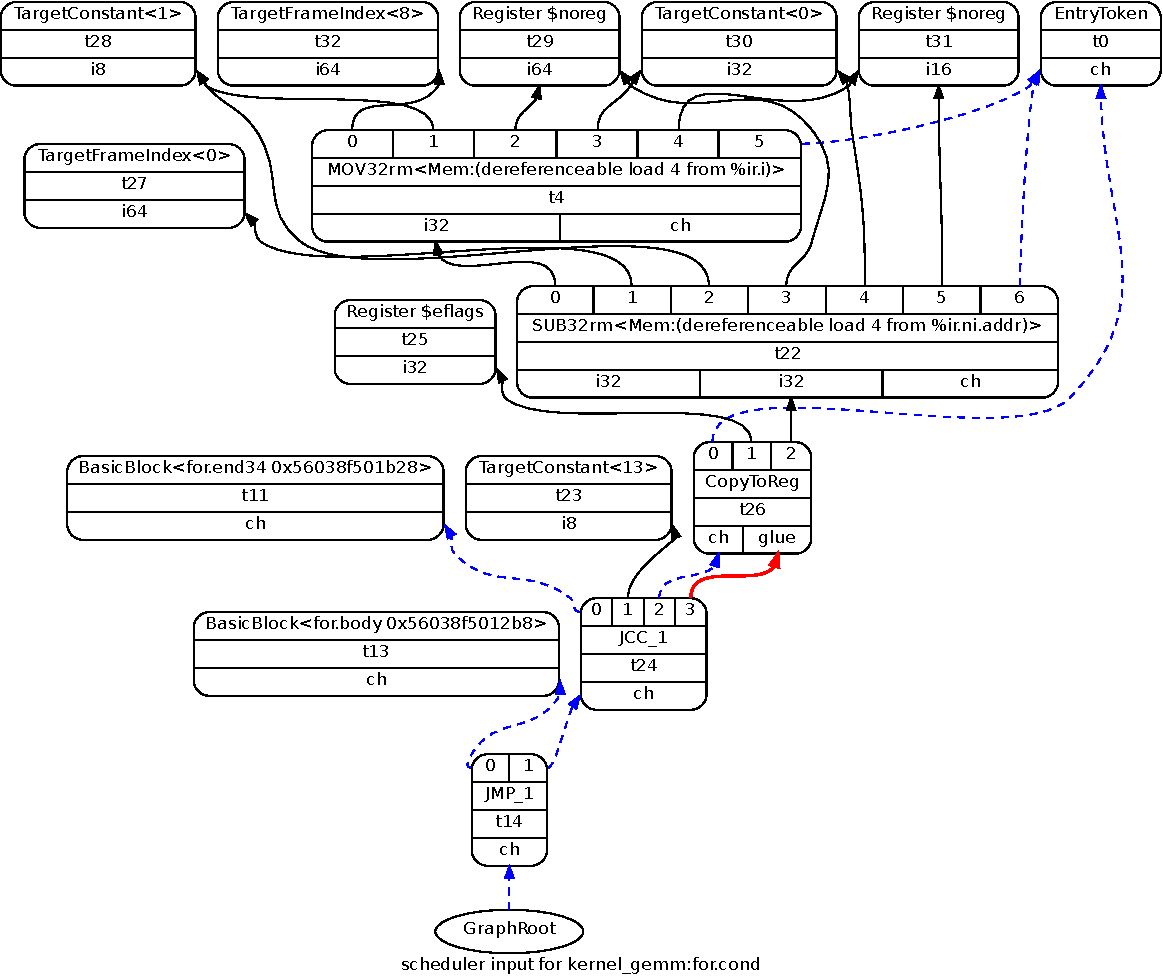
\includegraphics[width=\textwidth]{img/example-dag-crop.pdf}
    \caption[Example \aclu{dag} generated by LLVM]{Example \ac{dag} generated by LLVM. It shows the (AArch64) instructions defined by LLVM and the dependencies between the instructions.}
    \label{fig:bg:llvm-dag}
\end{figure}

Arrowed edges represent the dependencies between instructions.
The arrows point from a given instruction to one of its dependency instructions.
Three different types of edges exist that represent different types of dependencies:
\begin{itemize}
    \item Black: Represents a data flow dependency. That means that an instruction consumes the result of the previous instruction.
    \item Dashed Blue: This edge ensures that two unrelated instructions in terms of data flow remain scheduled in the correct order.
        In \Cref{fig:bg:llvm-dag}, the conditional jump instruction \lstinline|t24| must be scheduled before the unconditional jump instruction \lstinline|t14|, even though there is no data-flow dependency between these two.
    \item Red: This edge represents two instructions that must be scheduled together without any instructions between them.
\end{itemize}

The nodes in the LLVM \ac{dag} represent instructions.
Outgoing dependencies are numbered and placed in the top row.
If no dependencies exist, this row is missing.
The instruction name is written in the next node row, which is the top row if there are no outgoing dependency edges.
The next row shows an internally used instruction ID.
The generated output type of this instruction is placed in the bottom row. 
There are three possible values for the output type:
\begin{itemize}
    \item The datatype of the instructions result, \eg \lstinline|i32|, \lstinline|i64|, \lstinline|f32|, \lstinline|f64|, or \lstinline|v2f32|.
    \item \lstinline|ch|, which represents no data but is placed together with the dashed blue dependencies.
    \item \lstinline|glue| also does not represent any data but is placed together with the red dependencies.
\end{itemize}

Even though the instruction selection has already finished, there can still be LLVM pseudo instructions.
They are resolved in later stages.
The LLVM \ac{dag} always contains an \lstinline|EntryToken| pseudo instruction which gets always scheduled first.
Additionally, there is the \lstinline|GraphRoot| node at the bottom does not represent any instruction and will not get scheduled.
The \lstinline|BasicBlock| pseudo instructions represent the \lstinline|EntryToken| of another basic block.

\subsection{Instruction Scheduling}
The instruction scheduling happens in two phases in LLVM.
There is an instruction scheduling phase before register allocation (pre-RA) and after register allocation (post-RA).
LLVM makes the main scheduling decisions in the pre-RA phase.
The post-RA phase is only there to eliminate some small inefficiencies that can be detected, once the hardware registers are assigned.
When we speak of instruction scheduling in the context of LLVM, we mean the pre-RA phase from here on.

The maintainers of the LLVM framework are working on replacing the current pre-RA scheduling classes.
The new schedulers use the \lstinline|MIScheduler| class as their base.
Initially, instruction scheduling was integrated in the code of the instruction selection phase and worked on the \lstinline|ScheduleDAG| class.
We decided to base our work on the older implementation as it is still wider spread, and most production-used instruction schedulers are implemented in this manner.

There are already different instruction scheduler implementations that come with LLVM.
These can be used by configuring the \lstinline|llc| back-end with the command line option \lstinline|--pre-RA-sched=| and the possible choices:
\begin{itemize}
    \item \lstinline|vliw-td|: Scheduler for VLIW processors
    \item \lstinline|list-ilp|: List scheduler for balancing instruction-level parallelism and register pressure
    \item \lstinline|list-hybrid|: List scheduler for balancing latency and register pressure
    \item \lstinline|list-burr|: List scheduler for reducing register usage
    \item \lstinline|source|: Similar to \lstinline|list-burr|, but prefers the ordering from LLVM \ac{ir}
    \item \lstinline|linearize|: Does not schedule but returns instructions as they come in from LLVM \ac{ir}
    \item \lstinline|fast|: For compile-time optimized suboptimal scheduler
    \item \lstinline|default|: The best scheduler for the used target hardware
\end{itemize}
We use the \lstinline|default| scheduler as our baseline in all experiments.


\section{Data-Driven Methods}
\label{sec:bg:ml}
Throughout this thesis, we utilize data-driven methods for different tasks.
We use Monte Carlo Tree Search for finding good instruction schedules and to build a dataset.
We describe this method in \Cref{sec:bg:mcts}.
For learning how to generate good schedules for unseen basic blocks, we use Support Vector Machines and Neural Networks, which we explain in \Cref{sec:bg:svm} and \Cref{sec:bg:nn}.

\subsection{Monte Carlo Tree Search}
\label{sec:bg:mcts}
\ac{mcts}~\cite{abramson1990expected} is a randomized search method for optimal decisions.
When, \eg a computer's task is to play a board game, it has to make decisions, and from the outcome of previous decisions, it has to make new decisions.
This process continues until the game is over.
From the beginning of the game until the end, we can model the decision-making process as a decision tree.
For small games, like Tic Tac Toe, it is possible to use the trivial Minimax algorithm~\cite{neumann1928theorie}, which checks all possible paths in the decision tree.
However, for games like Chess, there are too many possible paths for a computer to simulate.
Another problem might be that the simulation itself is costly.
This process is too slow for the number of possible instruction schedules that exist for a typical basic block.

\ac{mcts} works by exploring one level of decisions  and finishing the path with random decisions.
When all decisions in a level were seen at least once, the algorithm will balance exploitation and exploration, which means it chooses the best possible decision most of the time.
However, sometimes it will choose another decision to learn more in an undiscovered part of the decision tree.
This balancing causes \ac{mcts} to learn how to extend the paths with better decisions.

We will explain the algorithm in more detail here.
The \ac{mcts} algorithm consists of four steps.
These are:
\begin{enumerate}
    \item Selection Phase:
        The algorithm starts from the root node of the \ac{mcts} tree and iterates down through the nodes by applying a child selection policy.
        It stops when it finds a node that has children, but not all children where visited yet.
        These nodes are called expandable nodes.
    \item Expansion Phase:
        The \ac{mcts} tree gets expanded by adding the available children to the selected node from the previous step.
        The new children are created with a view count of 0.
    \item Simulation Phase:
        From the selected node, the path through the \ac{mcts} tree will be filled with randomly chosen nodes until a terminal state is reached.
        In this phase, no nodes will be added to the tree.
        They will just be used to fill the path.
        This path through the \ac{mcts} tree gets evaluated, \eg by playing the board game with the decisions or in our case by checking the runtime of the instruction schedule.
    \item Backpropagation Phase:
        The evaluation of that path gets applied to the statistics of all the path's nodes.
\end{enumerate}
The node statistics are typically just two values.
First, the count of how many times a node was included in a simulation (view count).
The second value is the cumulated evaluation metric.
Typically, cumulated means the average value.
However, in our case, it is beneficial to use the maximum value instead of the average.
This was also mentioned in~\cite{bjornsson2009cadiaplayer} and generalized for single-player games.

The child selection policy, mentioned in the selection phase, is a strategy to find a path through the \ac{mcts} tree.
There are two possible extreme ways.
The first is to choose always the nodes with the lowest view count to find out more about nodes that we do not know much about.
This is known as exploration.
The opposite thing to do is always follow the node with the best metric, which is called exploitation.
These two aspects have to be balanced.
There are many ways to balance exploitation versus exploration, and it is a field of active research.
The standard policy for balancing is Upper Confidence Bounds for Trees (UCT)~\cite{kocsis2006bandit,kocsis2006improved}.

\subsection{Support Vector Regression}
\label{sec:bg:svm}
\ac{svm}~\cite{cortes1995support} is a robust classification algorithm.
There is also an extension for regression problems, which is called \ac{svr}~\cite{drucker1997support}.
We use the \ac{svr} model, but we will first briefly explain the classification model, as the regression model is based on this.

Originally, \ac{svm} is a model that gets trained to separate data points into two classes.
This model is then able to transfer what it has learned to new, unseen data points.
\ac{svm} does this by creating a hyperplane that separates the two classes of data points.
The goal is to maximize the margin between the hyperplane and all the datapoints, such that it separates the classes.
However, data is often not easily separable.
Therefore, \ac{svm} allows some data points inside of the margin area.

The \ac{svr} algorithm also tries to fit a hyperplane.
However, \ac{svr} tries to have as many data points as possible inside of the margin area.
This means that the hyperplane is located close to the data points.
Then, this hyperplane is used as the modeled function, not as a separation.

If the data points are not easily separable, the non-linear extension to the \ac{svm}, the Kernel-\ac{svm}, might help.
By applying the kernel-trick, the datapoints are mapped into a higher dimensional space.
This makes them easier separable.
The non-linearity might also help the \ac{svr} algorithm for learning non-linear functions.

\subsection{Neural Networks}
\label{sec:bg:nn}
% Importance of NN in the last decade
Much development in the machine learning field is based on artificial neural networks since the 2010s.
Especially, the computer vision and natural language processing fields profited from neural networks.
There are special types of neural networks for working on images which are called \ac{cnn}~\cite{lecun1998gradient}.
The weight that these networks learn are the weights of convolution operations.
Successful implementations of \acp{cnn} are, \eg~\cite{krizhevsky2012imagenet,he2016deep} on a image classification task.
Another important type of neural networks are Recurrent Neural Networks~\cite{rumelhart1985learning}.
These are often used in \ac{nlp} problems, \eg~\cite{graves2013speech,socher2013recursive}.
However, in this thesis, we use standard neural networks.

The foundations of this field date back to the 1950s~\cite{rosenblatt1958perceptron}.
With increasing computation power, more and more layers were added to the neural networks.
Machine learning with deep neural networks are often referred to as deep learning.

Neural networks are organized in layers of learned weights, which are called neurons.
Each layer function is wrapped by a non-linear activation function $a$.
This results in the mathematical formulation of a layer as
\begin{equation}
    O(X) = a(WX+b)
\end{equation}
with the neurons $W$, the bias $b$, and the input vector $X$.
The input can be either the input data if this is the first layer or the output of the previous layer in the neural network.

% Gradient Descent
To optimize neural networks, \ie learn the weights $W$, usually a gradient descent approach is used.
An error function is defined, which measures the distance between the prediction and the expected output.
Gradient descent adjusts the weights $W$ step by step in a direction that minimizes the error.

\chapter{Related Work}
\label{sec:rw}
In this chapter, we survey the existing relevant literature covering this thesis' topics. 
For instruction scheduling (\Cref{sec:rw:instruction-scheduling}) and register allocation (\Cref{sec:rw:register-allocation}), we first discuss classical approaches and continue with newer data-driven advancements.
Further, we discuss some other relevant works in the fields of machine learning-based compiler optimizations, runtime estimation, code feature extraction, and machine learning approaches on other scheduling tasks (\Cref{sec:rw:other}).
These are interesting because we use methods like this in our approach or they are closely related.

\section{Instruction Scheduling}
\label{sec:rw:instruction-scheduling}
\subsection{Classical Approaches}
Scheduling problems appear in many fields where tasks with dependencies and a cost need to be ordered for execution.
Therefore, general scheduling is a topic with much existing research.
Also, the research on instruction scheduling has a long history.

Some algorithms can generate perfect instruction schedules for simple situations with perfect information.
Architectures with only one functional unit and uniform instruction latencies fulfill the requirements.
The best-known algorithms in this field are the Sethi-Ullman labeling algorithm~\cite{sethi1970generation} and the work by \citeauthor{proebsting1991linear}~\cite{proebsting1991linear}.

However, these conditions are not present in modern processors, as discussed in \Cref{sec:bg:cpu}.
In more complex situations, the instruction scheduling problem is NP-complete~\cite{hennessy1983postpass}.
Modern processors use multiple pipelines to achieve instruction parallelism, see \Cref{sec:bg:cpu}.
Consequently, most instruction schedulers used nowadays are based on the list scheduling framework, which \citeauthor{landskov1980local}~\cite{landskov1980local} proposed.
The algorithms that follow this approach are better able to generate instruction schedules for pipelined processors.
\citeauthor{heller1961sequencing}~\cite{heller1961sequencing} published early work on how to approach instruction scheduling for these processors.
Further research on developments of list scheduling was published in~\cite{bernstein1991global,gibbons1986efficient,hennessy1983postpass}.

As elaborated in \Cref{sec:bg:cpu}, the available information on instruction latencies is often unreliable due to instruction-level parallelism and unpredictable memory latencies caused by cache hierarchies.
One way to approach this problem is balanced scheduling~\cite{kerns1993balanced,lo1995improving}.
Another proposed method was to use stochastic instruction scheduling~\cite{schielke2000stochastic}.

Instruction scheduling typically works on a basic block level.
This means that instruction schedulers cannot schedule transitions across basic blocks.
However, there is research on extending the scope to larger regions.
\citeauthor{fisher1981trace}~\cite{fisher1981trace} selected code paths in functions for instruction scheduling.
\citeauthor{bernstein1991global}~\cite{bernstein1991global} define regions of strongly connected code (\eg loops) and execute scheduling on this unit.
Superblock scheduling was proposed by \citeauthor{hwu1993superblock}~\cite{hwu1993superblock}.
A superblock consists of multiple consecutive basic blocks and thus can start execution from other instructions than the first one.

\subsection{Data-Driven Approaches}
List schedulers usually have multiple heuristics used to choose instructions from the list of available instructions.
The selection is based on a weighted sum of the heuristics.
The first work that combined data-driven methods with instruction scheduling is a patent by \citeauthor{tarsy1994method}~\cite{tarsy1994method}, filed in \citeyear{tarsy1994method}.
They optimize weights used in cost-based heuristics.
These heuristics are used in list scheduling for pipelined processors.

Similarly, \citeauthor{beaty1996using}~\cite{beaty1996using} published a work in \citeyear{beaty1996using} in which they used a genetic algorithm to learn weights for different heuristics.
They achieved a 5\% performance increase compared to a random scheduler on three architectures.

\citeauthor{moss1997learning}~\cite{moss1997learning} trained a function that picks one instruction over another when presented the previously scheduled instructions.
They use decision trees, look-up tables, ELF function approximations, and feed-forward neural networks.
The decision tree performs best and often finds the optimal schedule.
However, they only use simulations and limit the basic block length to ten instructions.

\citeauthor{mcgovern1999scheduling}~\cite{mcgovern1999scheduling,mcgovern2002building} propose a reinforcement learning and a search heuristic.
Their reinforcement learning heuristic sometimes found a better instruction schedule than their baseline.
The long-running search approach found a better instruction schedule every time.
However, their baseline was only a random instruction scheduler, and they have only used simulation results instead of using a state-of-the-art compiler and executing their benchmarks on hardware.

\citeauthor{russell2006learning}~\cite{russell2006learning} uses decision trees to create heuristics for improving instruction scheduling decisions.
They show that they generate better instruction schedules 7.8 times more often than the compared heuristics.
They also evaluate their work only on a simulator.

A newer work in this field was published by \citeauthor{jain2019learning}~\cite{jain2019learning}.
They train a neural network to imitate the instruction schedules by the GCC compiler.
However, the performance of the GCC instruction scheduler limits this approach’s performance.

We conclude that machine learning-based approaches mostly performed well in theory but only against weak random baselines.
The only work that we found that was actually evaluated on hardware was~\cite{beaty1996using}.

\section{Register Allocation}
\label{sec:rw:register-allocation}
We have discussed the implications of the instruction scheduling phase on register allocation in \Cref{sec:bg:compilers:backend}.
Their interdependence was also shown by \citeauthor{goodman1988code}~\cite{goodman1988code}.
\citeauthor{lavrov1962store}~\cite{lavrov1962store} showed the connection between the graph-coloring problem and register allocation and thus, the NP-completeness.
The first graph-coloring-based algorithm was implemented in a compiler by \citeauthor{chaitin1982register}~\cite{chaitin1982register}.

In the field of register allocation, also appeared research that builds the connection to data-driven methods.
\citeauthor{das2019deep}~\cite{das2019deep} use a deep learning approach to solve the graph coloring problem.
The newer and naturally better fitting approach with graph neural networks was used by \citeauthor{lemos2019graph}~\cite{lemos2019graph} to solve the graph coloring problem. 

\section{Related Areas}
\label{sec:rw:other}
\subsection{Compiler Optimizations with Machine Learning}
Machine learning approaches are also applied to optimize other parts of the compilation process.
\citeauthor{mammadli2020static}~\cite{mammadli2020static} and \citeauthor{huang2019autophase}~\cite{huang2019autophase} successfully apply deep reinforcement learning to the phase-ordering problem.
Phase-ordering means to select the compiler's optimization passes and define its execution order (see \Cref{sec:bg:compilers:optimizer} for information on the optimization phase).
Deep reinforcement learning was also used by \citeauthor{haj2020neurovectorizer}~\cite{haj2020neurovectorizer} to translate loops into vector processing instructions (SIMD).
\citeauthor{wang2009mapping}~\cite{wang2009mapping} used machine learning to predict the optimal number of threads and the optimal scheduling policy for OpenMP parallelized loops.
We refer to the surveys~\cite{wang2018machine,ashouri2018survey} for more literature.

\subsection{Runtime Estimation}
\label{sec:rw:other:runtime}
There are various tools for throughput and runtime estimation, like Ithemal~\cite{mendis2019ithemal}, llvm-mca\footnote{https://llvm.org/docs/CommandGuide/llvm-mca.html}, and Intel Architecture Code Analyzer (IACA)\footnote{https://software.intel.com/content/www/us/en/develop/articles/intel-architecture-code-analyzer.html}.
However, the listed tools only work with the x86 architecture, which we do not use.
The research projects and open-source estimators might be extended to other hardware architectures.
Especially the Ithemal~\cite{mendis2019ithemal} project is interesting as they use a neural network to predict the runtime from the basic block.
That means they learned to extract relevant features from the basic blocks instructions.

\subsection{Feature Extraction from Code}
The previously cited works on data-driven machine learning optimizations have or might benefit from research whose goal is to extract features from code automatically.
A similar approach to the word2vec~\cite{mikolov2013efficient} approach in the \ac{nlp} area was proposed by~\cite{ben2018neural,alon2019code2vec}.
\citeauthor{cummins2021programl}~\cite{cummins2021programl} developed a method to extract features from code based on graph structures.
The work proposed by \citeauthor{brauckmann2020compiler}~\cite{brauckmann2020compiler} works similarly -- they also work on graph structures and use graph neural networks to extract features.

\subsection{Other Scheduling Tasks with Machine Learning}
\citeauthor{mao2019learning}~\cite{mao2019learning} have used a deep reinforcement learning approach to schedule data-processing jobs onto computing clusters.
This work is interesting because the jobs have dependencies on each other, represented in a \ac{dag}, just like the instructions in the instruction scheduling problem.

\IMRADlabel{methods}
\chapter{Approach}
\todo{Why are we using a data-driven / machine learning approach? Show that it is complicated to do it by hand. Also write why not to do auto-tuning.}

\begin{figure}
    \centering
    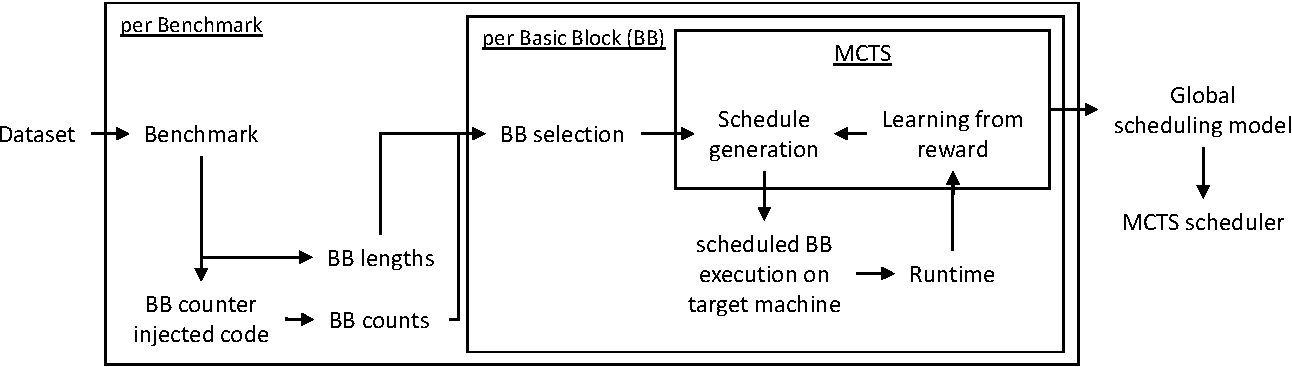
\includegraphics[width=\textwidth]{img/ppt/approach_overview-crop.pdf}
    \caption[Overview of the approach]{Overview of the overall approach. 
    The process covers the selection of basic blocks, the instruction schedule generation, the execution model, the learning process and the derivation of the final scheduler.}
    \label{fig:approach:overview}
\end{figure}
In the rest of this chapter, we will present the approach used for this thesis (compare~\cref{fig:approach:overview}).
We start with an overview of the benchmark programs we used~(\cref{sec:approach:dataset}).
Then we discuss the importance of basic blocks for instruction scheduling in general and our approach specifically~(\cref{sec:approach:basicblock}).
That is followed by explaining the \ac{mcts} approach~(\cref{subsec:approach:ml:mcts}).
Eventually, we introduce how we combine individual \ac{mcts} models into a global model~(\cref{subsec:approach:ml:global}) and derive an applicable scheduler~(\cref{sec:approach:ml-scheduler}).

\section{Dataset}
\label{sec:approach:dataset}
For our experiments, we use benchmarks from the LLVM project called LLVM Test Suite~\footnote{\url{https://llvm.org/docs/TestSuiteGuide.html}}.
The test suite contains benchmarks in the following categories
\begin{itemize}
    \item Single-Source --- built from a single C/C++ source file
    \item Multi-Source --- built from multiple C/C++ source files
    \item Micro-Benchmarks --- seperate functions, that are executed by google-benchmark
    \item Bitcode --- tests that are written in LLVM bitcode
    \item CTMark --- symbolic links to the other benchmarks to measure compilation performance
\end{itemize}
We select the 273 benchmarks from the Single-Source and Multi-Source categories for our experiments.
\todo{Add table?}
The benchmarks are all written in C or C++.
These categories contain benchmarks that are compiled from a single source file or multiple source files, respectively.
In addition, the test suite contains more benchmarks that are not relevant to our experiments or took too long to integrate.

\subsection{Modified build process}
\label{sec:approach:build_process}
The test suite comes with Makefile's and CMake configuration to automatically build all the benchmarks.
However, these are not sufficient for our approach.
We need a modified build process for all the benchmarks because we are manipulating it in several cases.
Furthermore, the compilation cannot be done with a single command because not all arguments of the separate compilation steps are available in the main compiler.
We execute the front-end, optimization, and back-end phase separately to have complete control over the build process.

We have to set some compiler arguments to make the LLVM compiler front-end eject LLVM \ac{ir} instead of compiling the program completely.
For C programs we use \lstinline{clang}~\footnote{\url{https://clang.llvm.org/}} and for C++ programs we use \lstinline{clang++}.
However, the compiler arguments are the same.
We pass the following arguments to the front-end:
\begin{itemize}
    \item \lstinline{-O0}: to prevent optimization in this first step
    \item \lstinline{-Xclang -disable-O0-optnone}: the \lstinline{-O0} flag alone also prevents optimization in further steps, which is not what we want
    \item \lstinline{-S -emit-llvm}: to emit LLVM \ac{ir} for further processing --- instead of compiling the program completely
\end{itemize}

The LLVM optimizer \lstinline{opt}~\footnote{\url{https://llvm.org/docs/CommandGuide/opt.html}} gives a choice to select one of the predefined optimization levels or select specific optimizer runs.
When we compile a benchmark for measuring the runtime, we only use the flag \lstinline{-O3} for optimizing the LLVM \ac{ir}.
The LLVM framework makes it easy to implement new optimizer passes.
We do this to count how often a basic block is executed (see \cref{sec:approach:basicblock:selection}) and measure a function's execution time (see \cref{sec:approach:datageneration:runtime:function}).

We manipulate the instruction scheduling by adjusting how we call the compiler back-end.
The LLVM static compiler implements two instruction schedulers before the register allocation and one after the register allocation.
The former inherit either from the C++ class \lstinline{SelectionDAG} or from \lstinline{MIScheduler}.
Which one will be executed by the compiler depends on the target architecture. 
It is also possible that the compiler executes both.

We manipulate the back-end by passing arguments to the LLVM static compiler \lstinline{llc}~\footnote{\url{https://llvm.org/docs/CommandGuide/llc.html}}.
This program represents the back-end phase and executes the instruction scheduling.
We use the following arguments for the back-end:
\begin{itemize}
    \item \lstinline{--pre-RA-sched=}: to select our new \lstinline{SelectionDAG} schedulers for the pre-register-allocation phase
    \item \lstinline{--misched-cutoff=0}: to disable the \lstinline{MIScheduler}
    \item \lstinline{--disable-post-ra}: to disable the post-register-allocation scheduler
\end{itemize}

We analyze the CMake configurations and extract required compiler arguments on a per benchmark level.
We categorize the extracted arguments into front-end, optimizer, and back-end phases.
Finally, we append them to the previously described arguments in the respective compilation phase.

We also analyze the test suite for execution arguments.
For example, some benchmarks read data from files or require arguments when calling them.
To execute them, we generate a shell script that calls the compiled benchmark with the required arguments.

\section{Basic Block --- scheduling unit}
\label{sec:approach:basicblock}
Even though there exists some research on instruction scheduling on more extensive units, most compilers schedule instructions on a per basic block level.
This is also true for the LLVM compiler framework.
The advantage of this is that the limited scope avoids complicated situations and thus simplifies the scheduling problem.
For Example, do not have to deal with jump instructions.

Consequently, we also choose the basic block as the unit for instruction scheduling.
That means that we execute our experiments on individual basic blocks and learn to schedule individual basic blocks.
Later, we combine the models to generalize the knowledge.
We describe this process in detail in \cref{sec:approach:ml}.

\subsection{Selection process}
\label{sec:approach:basicblock:selection}
Not all basic blocks provide an equal value to our experiments.
It also consumes too much time to work on all the basic blocks within the scope of this thesis (\eg compilation time, execution time, machine learning time).
Therefore, we sort our basic blocks by heuristics. 
From this list, we select as many as we need and can handle in our experiments.
We designed three heuristics which we will explain in the following paragraphs.
See \cref{tab:approach:bb_heuristics} for an example overview.

\begin{table}
    \centering
    \begin{tabular}{@{}llrrr@{}}
        \toprule
        Function & Basic Block & Length & \(\#\) Executions & Product \\
        \midrule
        kernel\_floyd\_warshall\_StrictFP & for.body6 & 23 & 536,870,912 & 12,348,030,976 \\
        kernel\_floyd\_warshall & for.body6 & 23 & 536,870,912 & 12,348,030,976 \\
        print\_element & entry & 25 & 1,048,576 & 26,214,400 \\
        kernel\_floyd\_warshall\_StrictFP & for.cond4.preheader & 17 & 1,048,576 & 17,825,792 \\
        \(\cdots\) & \(\cdots\) & \(\cdots\) & \(\cdots\) & \(\cdots\) \\
        xmalloc & entry & 8 & 2 & 16 \\
        main & entry & 11 & 1 & 11 \\
        \bottomrule
    \end{tabular}
    \caption[Basic block heuristics for the floyd-warshall benchmark]
    {
        The tables shows an excerpt of the basic block heuristics (see \cref{sec:approach:basicblock:selection}) for the floyd-warshall benchmark. 
        The basic blocks are sorted by the last heuristic, which is the product of the length and execution count. 
        From this list the table shows the top four and last two basic blocks in the benchmark.
    }
    \label{tab:approach:bb_heuristics}
\end{table}

\subsubsection{Longest basic blocks}
The number of instructions in a basic block correlates with the number of possible schedules.
Consequently, we can learn more from a basic block when there are more different scheduling situations available.
For example, we will see more scheduling situations in a basic block containing 20 instructions than in a basic block containing only three instructions.

We implemented a hook into the LLVM framework to count the number of instructions in a basic block.
This hook prints the number of instructions in each basic block during the compilation process.
From this output, we put together a list with all basic blocks and their lengths (see \cref{tab:approach:bb_heuristics}).

\subsubsection{Most executed basic blocks}
Some basic blocks are significantly more often executed than others.
For example, basic blocks in the bodies of loops run often.
A basic block in the error checking code of the beginning of a program might only execute once.
Often executed basic blocks influence the overall runtime a lot.
Hence, we are more interested in optimizing these.
See \cref{tab:approach:bb_heuristics} for an example.

We implemented a LLVM optimizer pass for injecting counters into a program.
Optimizer passes take LLVM \ac{ir} files as input and output the code in the same file format.
Our pass injects one global 64 bit counter variable for each basic block into the code.
Next, the pass adds instructions into the beginning of each basic block, which increase the corresponding counter by one.
At the end of the main function the pass adds a format string and injects a call to the \lstinline{printf} function to print all the counter values and corresponding basic block names.

The optimizer pass must be compiled with the LLVM framework.
We include the optimizer pass into our build process (see \cref{sec:approach:build_process}).
There, we add a call to the LLVM optimizer \lstinline{opt} with the argument \mbox{\lstinline{-passes=dyn-bb-count}}.
To actually get the counts, we build a benchmark with this optimizer pass and and execute it.
The benchmark will then print the counter values.

\subsubsection{Most executed and longest basic blocks}
The previous two heuristics are helpful on their own, but we are most interested in basic blocks that combine the two aspects.
For example, the most executed basic block can still come from a very simple loop with few instructions in the loop body.
We compute the product of the two heuristics to get a combined heuristic.

\section{Learning to schedule}
\label{sec:approach:ml}
\subsection{Local MCTS model}
\label{subsec:approach:ml:mcts}
\subsection{Global model}
\label{subsec:approach:ml:global}

\section{Data generation}
We cannot build our data-driven models (see \cref{sec:approach:ml}) directly from our dataset, described in \cref{sec:approach:dataset}.
Learning from this dataset requires some transformation from the code to a metric we are interested in.
Many metrics can be chosen for optimization \eg runtime, energy consumption, cache misses, processor stalls.
We focus on optimizing the instruction scheduling for fast runtimes.
To generate data for our MCTS approach we need a mapping from instruction schedules to runtimes.
Therefore, we compile the code with varying instruction schedules and execute it to measure its runtime.
We discuss various aspects of this in the remainder of this section.

\subsection{Runtime measurement unit}
It would be optimal to just measure the the scheduled instructions with perfect precision and reliability.
\subsubsection{Basic Block}
\begin{itemize}
    \item What: Measuring the basic block itself is complicated
    \item Why: we need very precise time measurements
    \item How: the typical length of a basic block ranges from a hand full of instructions to a few dozens
    \todo{Plot basic block length distribution}
\end{itemize}
\subsubsection{Function}
\label{sec:approach:datageneration:runtime:function}
A specific basic block of a function might be executed multiple times during function execution.
In this situation, this is relevant in to different aspects.

% \begin{itemize}
%     \item What: Advantage: BB is executed multiple times, so its runtime is easier to measure
%     \item Why: 
%     \item How: 
% \end{itemize}
We are more interested in speedups, rather than precise execution times.


\begin{itemize}
    \item What: Measure the function which contains the basic block is bad in general
    \item Why: Different paths could be taken throught the function, e.g. if-else, loops
    \item How: 
\end{itemize}
\begin{itemize}
    \item What: In this case it is okay
    \item Why: the benchmarks are deterministic, each path is taken the same number of times between executions
    \item How: 
\end{itemize}
\subsubsection{Program}
\begin{itemize}
    \item What: Measure the execution time of the whole program
    \item Why: Easy, but unreliable because of IO operations and other noise (e.g. OS), we are only interested in a small fraction of the code
    \item How: 
    \todo{Show visualization}
\end{itemize}

\subsection{Runtime measurement methods}
\todo{Could add little experiment where we compare hardware timers vs OS access}
\subsubsection{Profiling}
\begin{itemize}
    \item What: Profilers are a bad choice for measuring precise runtimes
    \item Why: They are just not designed for it, they serve other purposes.
        Profilers are making snapshots of the running system to measure performance. 
        There is no measurement from point A to point B which leads to inaccuracies
    \item How: Read e.g. the paper of gperf \cite{graham1982gprof}
\end{itemize}
\subsubsection{Operating system methods}
% In linux(C): clock_gettime().
% Windows: QueryPerformanceCounter().
% C++: std::high_resolution_clock().
These might return different clocks depending on the used hardware.
Returns the time from the hardware the OS runs on.
Has overhead but also handles problems.
Typically best for measurements in microseconds range and longer.
\subsubsection{Hardware performance counters}
Accessed by assembly instructions.
% x86: 'rdtsc' Saves current value into EDX:EAX registers
% ARM32: mrc p15m, 0, \%0, c15, c12, 1
% AARCH64: mrs \%0, PMCCNTR_EL0
% Aurora: fencei; smir \%0, \%usrcc
Measurements in CPU cycles.
Lowest overhead available.
Access might be protected (Linux module required).
\subsection{Basic block isolation}
\subsubsection{Basic block extraction}
How to get the assembly (compilation process).
Problems: function calls (remove), jumps(only in last instr, remove), load/access (memory access, readress to stack variable)
\todo{Create table with removed instructions}
\subsubsection{Isolated basic block execution}
From extracted basic block create inline assembly with stack variable. Now executable from C/C++.
Warmup 100 runs. Timings 1000 runs. 
\subsection{Computing rewards from runtimes}
There are some outliers in the runtimes. Sort runtimes, cutoff lower and upper 5\% of the runtimes to remove outliers and compute avg of the rest.
What could be reasons for outliers?
Show some distributions of measurements to justify why we are throwing away data.

\section{Application of the learned model}
\label{sec:approach:ml-scheduler}

% Probably wrong place here, but compare approach with auto-tuning approach.
% Why not use auto-tuning? Search space size, and lack of generalization could be a reason

% \section{Breaking down the problem (maybe just chapter introduction)}
% \begin{itemize}
%     \item Schedulers run on basic blocks -> Select the most executed (hottest) BB's
% \end{itemize}

% \section{Experimentation Pipeline}
% Explain and illustrate the pipeline incl. injection of timers and counters

% \section{Benchmarking}
% \begin{itemize}
%     \item Benchmarking methods: Instrumentation, sampling -> only instrumentation makes sense here. Justify this with instrumentation vs. sampling results (our timing vs. perf timing)
%     \item Where to inject timer in BB DAG
%     \begin{itemize}
%         \item We only want to measure optimized code, but not too kleinteilig because of lacking accuracy. Problematic code is IO code
%         \item Time whole function?
%         \item Time only relevant BB's with surrounding ones (e.g., loop headers) -> Where exactly place the the timer
%         \item Provide data and examples to demonstrate decision making
%     \end{itemize} 
% \end{itemize}
% \subsection{Implementation}
% Injection of the \lstinline[language=C++]{std::chrono::high_resolution_clock}

% \section{Training setup}
% Compile with default scheduler and measure its runtime.
% Compile with our scheduler, execute the program, measure the runtime and use it to train the agent.

% \section{MCTS}
% \subsection{Tree Modeling}
% We probably want to model the interdependence between instructions. 
% But depending on the benchmark programs, only a small fraction of possible edges between instructions are available.

% \eg When in the benchmark a MOV was scheduled and after that, there are only SUB and ADD.
% We cannot schedule another MOV even though that might be the optimal schedule.

% This problem must be addressed somehow.
% There are different possibilities:
% \begin{itemize}
%     \item Declare all the states with their possible successors to different states.
%     The problem with this approach is that the number of states gets very high and most states are visited rarely, possibly only in the given benchmark/basic-block.
%     \item Probablistic Policy like in RL. (Does that exist for MCTS?)
%     This might solve the problem with unavailable edges, but it does not help with learning at all because the agent would have to learn which instructions are available, too.
%     Which is not what we want.
% \end{itemize}
\IMRADlabel{results}
\IMRADlabel{discussion}
\chapter{Evaluation}
In this chapter we explain how we used the system described in \Cref{sec:approach} to evaluate its performance.
First, we review the results of the \ac{mcts} approach in \Cref{sec:eval:mcts}.
Followingly, we evaluate if we can use the results of the \ac{mcts} approach to learn to generate good schedules with supervised learning methods in \Cref{sec:eval:supervised}.

\section{Hardware selection}
\label{sec:eval:hw}
The moste relevant hardware feature of processors when working on instruction scheduling is the instruction pipeline.
We are specifically interested in the fact if a instruction pipeline is a in-order or out-of-order pipeline (\Cref{sec:bg:superscalar-cpu}).
In-order processors execute the instructions in the schedule that is written in the executable file.
A out-of-order processor might reschedule the instructions in hardware.

For our experiments we have selected two different types of processors, one of each type:
\begin{itemize}
    \item 
    % \subsubsection{AArch64}
    The AArch64 hardware architecture is a 64-bit ARM architecture with a in-order superscalar pipeline.
    A \ac{cpu} that implements this hardware, and that we use for our experiment is the Arm Cortex-A53.
    We use this \ac{cpu} in the RaspberryPi 3 Model B with a Ubuntu 20.04.
    \todo{Correct Ubuntu version?}
    
    \item
    % \subsubsection{\aurora}
    The second processor is the \aurora vector processor that implements a out-of-order superscalar pipeline.
    This processor is installed via a PCI-Express slot.
\end{itemize}
    
\section{Approach Validation}
Before starting to optimize a process, it is useful to validate that there is potential for any optimizations.
Therefore, we show, that different instruction schedules can indeed have different runtimes on our target hardware.
The approach of this experiment is differs from the other experiments because it is an early experiment that took place before our pipeline was developed.
\todo{Is this sentence useful /okay?}

% select longest bb per benchmark
% longest might have the most possible schedule, so more variation in the random schedules
\Cref{sec:approach:dataset} describes the selection of benchmarks from the LLVM Test Suite.
For this experiment we select one basic block per benchmark, for which we modify its instruction schedule.
For the selection of basic blocks we use the heuristic that balances between the most executions and the longest basic blocks, which is discussed in \Cref{sec:approach:basicblock:selection}.
A high number of instructions in a basic block is typically a good indicator for a high number of possible instruction schedules for that basic block. 
A high number of executions ensures that the basic block has a high impact on the runtime of the function that it contains.

% measure the function runtime
% we measure the runtime of the function (implemented llvm passes)
% talk about impact on measurements.
We executed this experiment in a early stage and did not have a basic block extraction pipeline nor means to measure the execution time of a single basic block.
Therefore, we must execute the whole benchmark with the modified instruction schedule of a single basic block.
However, measuring the runtime of the whole benchmark, includes the execution of much overhead code, that we are not interested in.
Thus, we measure the runtime of the function that contains the basic block of interest.
This corresponds to the third method in \Cref{fig:approach:runtime_scopes}.

We implement a pass for the LLVM optimizer, to measure the runtime of a single function.
\todo{Put into approach chapter?}
The pass searches for the function that contains the selected basic block.
Then, it injects calls to the timer functions of the C++ standard library (\lstinline|std::high_resolution_clock::now|).
The calls are injected at the beginning of the given function and right before the return statement.
It injects a compilation-unit-wide global variable, and stores the measurements into this variable.
In the destructor of that compilation-unit, the pass injects code to print all the measurements.

% generate 10 different random schedules 
% do that twice
To generate different different instruction schedules, we choose the simple approach of generating random schedules.
Our random instruction scheduler works on top of a basic list scheduler.
This means, that the list scheduler selects the instructions that are ready for scheduling, and our random scheduler randomly selects one of them.
This is done until no more instructions are left.
We set the seed of the random number generator for reproducibility.

We generate instruction schedules with the seeds 0-10 for each selected basic block, \ie we generate 11 instruction schedules per basic block.
The basic block of interest might execute multiple times in the measured function for reasons discussed in \Cref{sec:approach:runtime-measurement-unit}.
We choose the shortest measured runtime per benchmark run, to ensure that we use the same execution path in our measurements.
To check that the runtime measurements are reproducible, we run the each generated instruction schedule two times.

% evaluate
We have run this experiment on the two processors described in \Cref{sec:eval:hw}.
\Cref{fig:eval:rndm:aarch64} shows a selection of experiment results.
The plots show the runtimes grouped by the different seeds for the random instruction scheduler.
Runtimes that differ between two runs more than 5\% are marked as outliers and plotted in gray.
\Crefrange*{fig:eval:rndm:aarch64:a}{fig:eval:rndm:aarch64:d} show examples where different runtimes are clearly observable for different instruction schedules.
However, this was not always observable.
\Cref{fig:eval:rndm:aarch64:e} and \Cref{fig:eval:rndm:aarch64:f} show examples where no differnce in the runtime was observable.
The average coeffecient of variation over the basic blocks is 0.035.
In summary, we see that different instruction schedules can generate measurable differences in the runtime.
This means that there is potential for improvements.
\begin{figure}
    \begin{subfigure}{0.45\textwidth}
        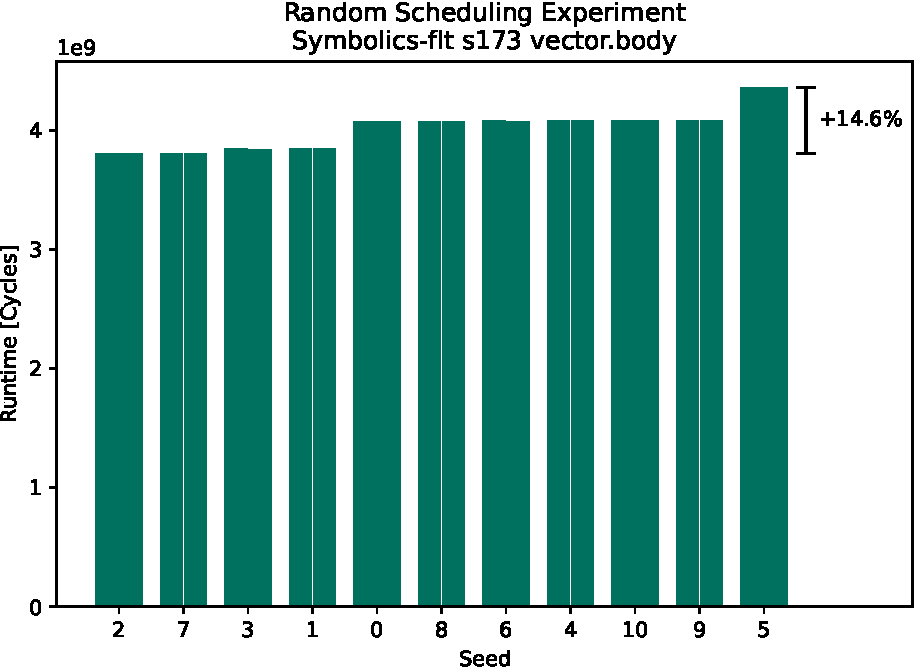
\includegraphics[width=\textwidth]{img/random-scheduling-experiment-pi-collected/Symbolics-flt-crop.pdf}
        \caption{}
        \label{fig:eval:rndm:aarch64:a}
    \end{subfigure}
    \hfill
    \begin{subfigure}{0.45\textwidth}
        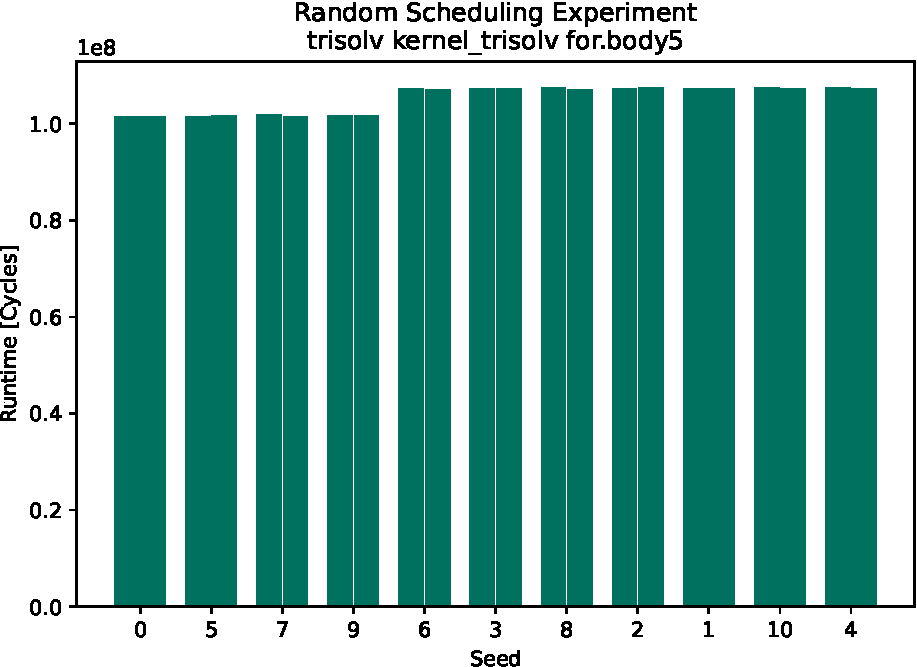
\includegraphics[width=\textwidth]{img/random-scheduling-experiment-pi-collected/trisolv-crop.pdf}
        \caption{}
        \label{fig:eval:rndm:aarch64:b}
    \end{subfigure}
    \begin{subfigure}{0.45\textwidth}
        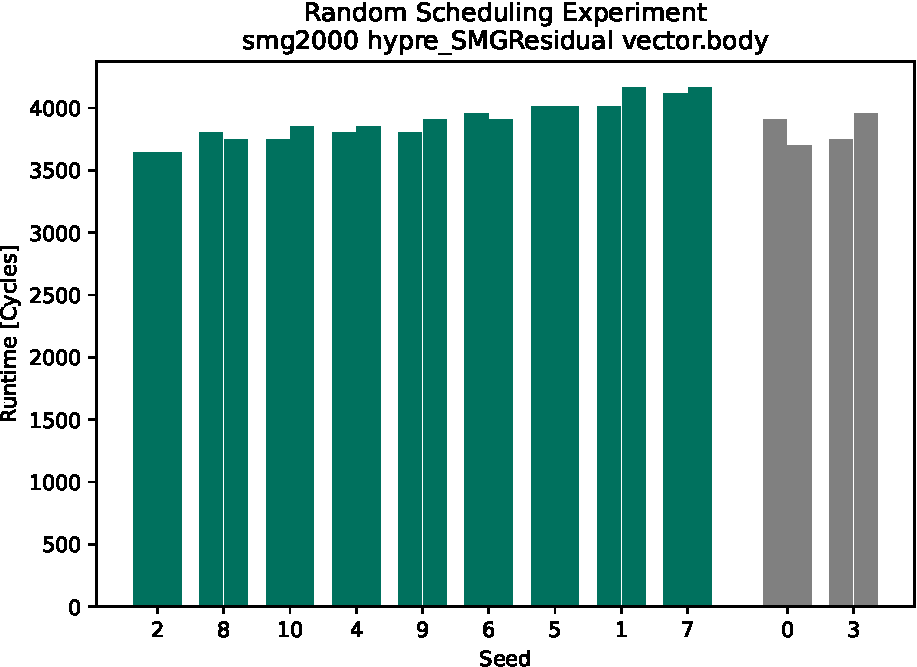
\includegraphics[width=\textwidth]{img/random-scheduling-experiment-pi-collected/smg2000-crop.pdf}
        \caption{}
        \label{fig:eval:rndm:aarch64:c}
    \end{subfigure}
    \hfill
    \begin{subfigure}{0.45\textwidth}
        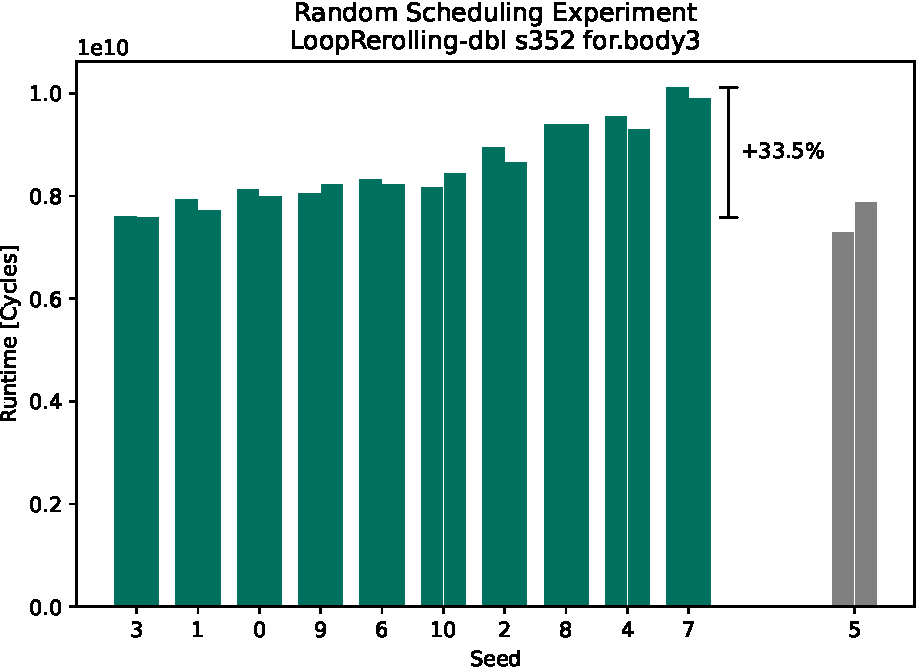
\includegraphics[width=\textwidth]{img/random-scheduling-experiment-pi-collected/LoopRerolling-dbl-crop.pdf}
        \caption{}
        \label{fig:eval:rndm:aarch64:d}
    \end{subfigure}
    \begin{subfigure}{0.45\textwidth}
        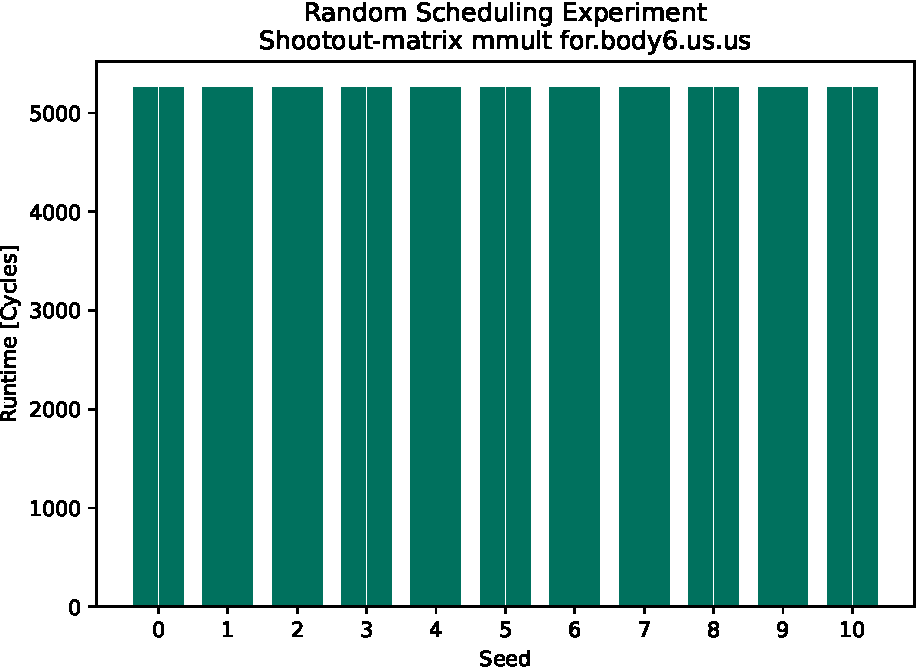
\includegraphics[width=\textwidth]{img/random-scheduling-experiment-pi-collected/Shootout-matrix-crop.pdf}
        \caption{}
        \label{fig:eval:rndm:aarch64:e}
    \end{subfigure}
    \hfill
    \begin{subfigure}{0.45\textwidth}
        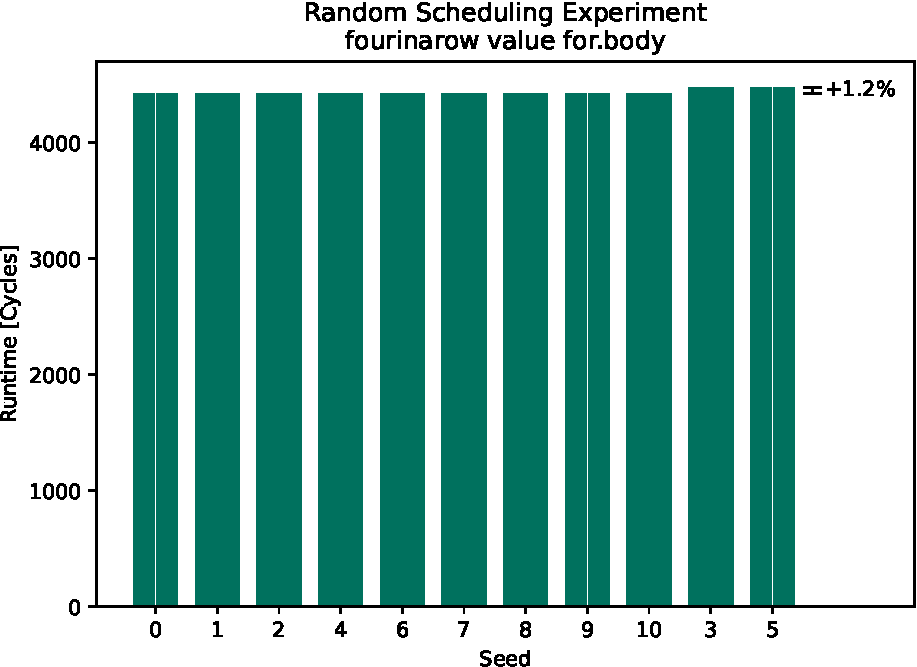
\includegraphics[width=\textwidth]{img/random-scheduling-experiment-pi-collected/fourinarow-crop.pdf}
        \caption{}
        \label{fig:eval:rndm:aarch64:f}
    \end{subfigure}
    \caption[Random Scheduling Experiment on AArch64]{Random Scheduling Experiment on AArch64:
    The bars show the runtime of a function with a random instruction schedule.
    The two runs of the instruction schedule are grouped together.
    Two runs that differ more than 5\% are marked as outliers and plotted in gray.}
    \label{fig:eval:rndm:aarch64}
\end{figure}

\Cref{fig:eval:rndm:aurora} shows a similar selection for the same experiment on the \aurora processor.
We can observe a similar outcome of the experiment.
However, as this processor cannot be interrupted by the \ac{os}, the runtimes are more stable between two runs.
No measurements in the whole example where marked as outliers.
The average coeffecient of variation over the basic blocks is 0.046.
In summary, we observe potential for optimizations on this processor.
\begin{figure}
    \begin{subfigure}{0.45\textwidth}
        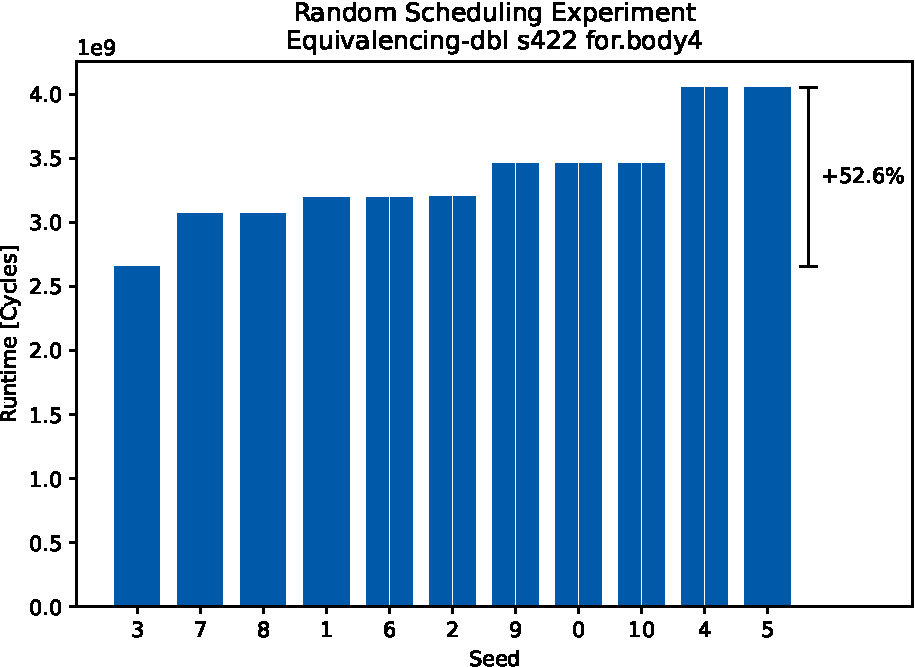
\includegraphics[width=\textwidth]{img/random-scheduling-experiment-aurora-collected/Equivalencing-dbl-crop.pdf}
        \caption{}
        \label{fig:eval:rndm:aurora:a}
    \end{subfigure}
    \hfill
    \begin{subfigure}{0.45\textwidth}
        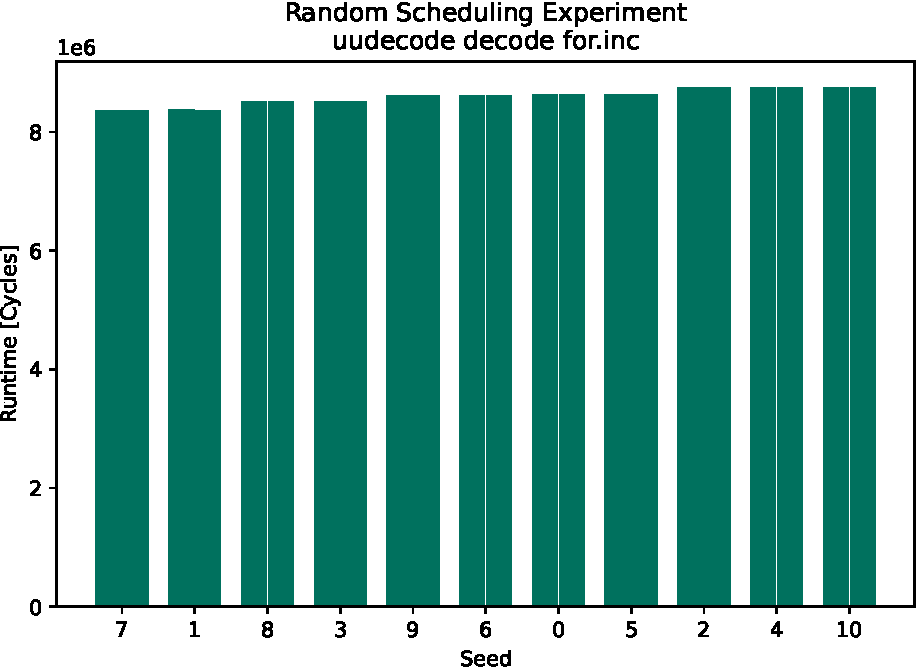
\includegraphics[width=\textwidth]{img/random-scheduling-experiment-aurora-collected/uudecode-crop.pdf}
        \caption{}
        \label{fig:eval:rndm:aurora:b}
    \end{subfigure}
    \begin{subfigure}{0.45\textwidth}
        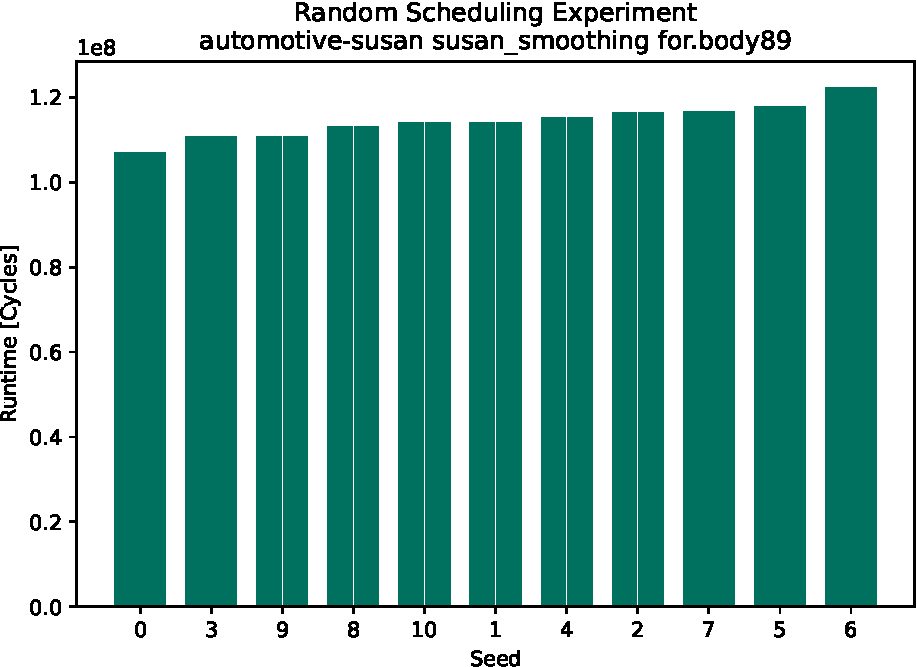
\includegraphics[width=\textwidth]{img/random-scheduling-experiment-aurora-collected/automotive-susan-crop.pdf}
        \caption{}
        \label{fig:eval:rndm:aurora:c}
    \end{subfigure}
    \hfill
    \begin{subfigure}{0.45\textwidth}
        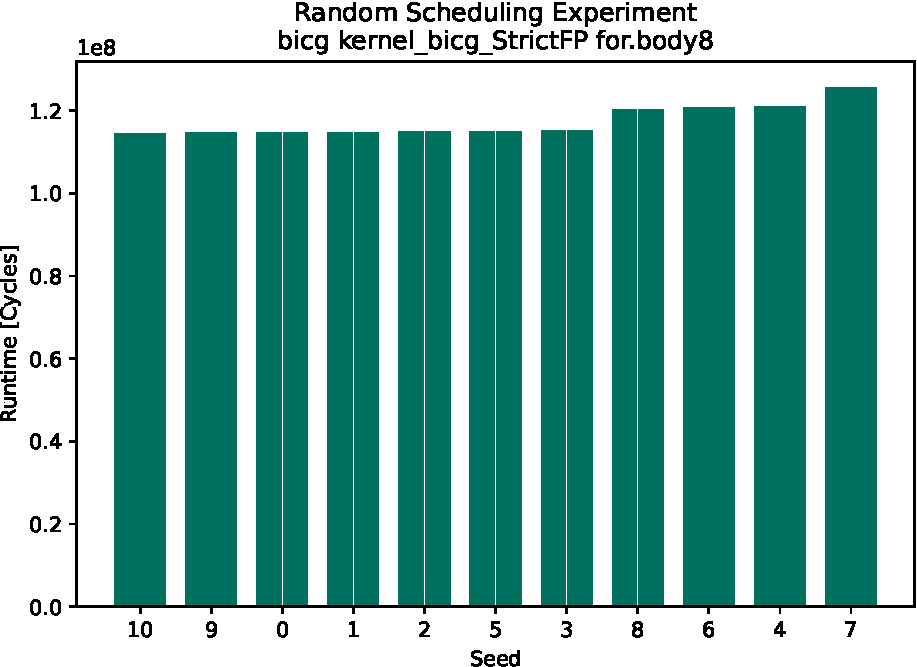
\includegraphics[width=\textwidth]{img/random-scheduling-experiment-aurora-collected/bicg-crop.pdf}
        \caption{}
        \label{fig:eval:rndm:aurora:d}
    \end{subfigure}
    \begin{subfigure}{0.45\textwidth}
        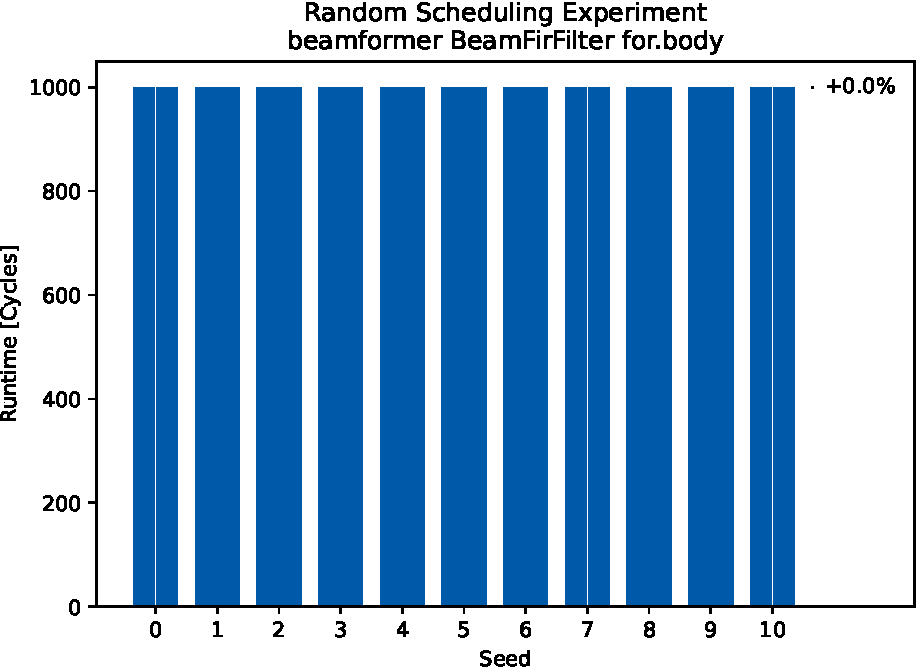
\includegraphics[width=\textwidth]{img/random-scheduling-experiment-aurora-collected/beamformer-crop.pdf}
        \caption{}
        \label{fig:eval:rndm:aurora:e}
    \end{subfigure}
    \hfill
    \begin{subfigure}{0.45\textwidth}
        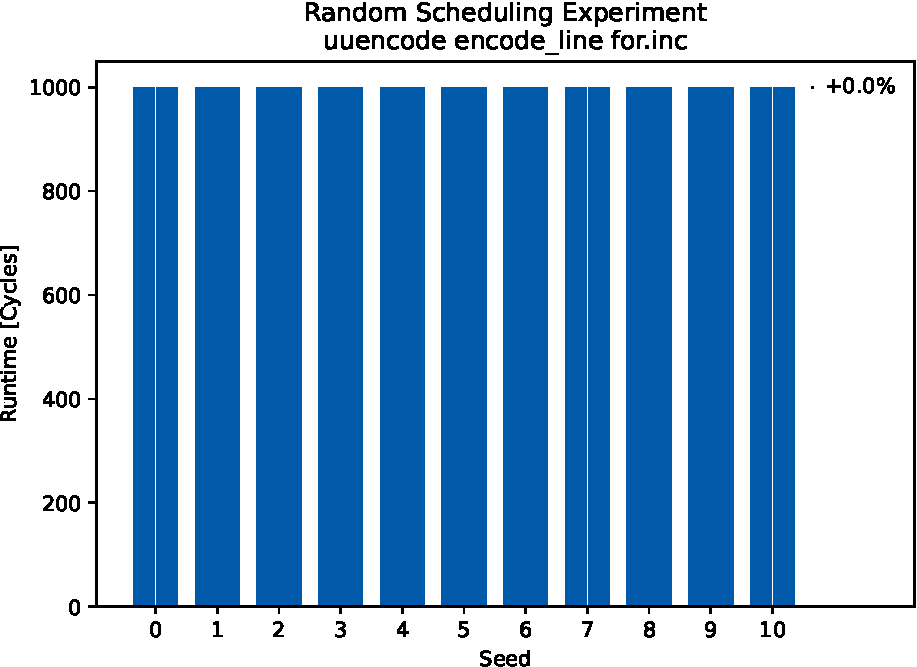
\includegraphics[width=\textwidth]{img/random-scheduling-experiment-aurora-collected/uuencode-crop.pdf}
        \caption{}
        \label{fig:eval:rndm:aurora:f}
    \end{subfigure}
    \caption[Random Scheduling Experiment on \aurora]{Random Scheduling Experiment on \aurora:
    The bars show the runtime of a function with a random instruction schedule.
    The two runs of the instruction schedule are grouped together.
    Two runs that differ more than 5\% are marked as outliers.
    However, this processor did not produce any outliers in our experiment.}
    \label{fig:eval:rndm:aurora}
\end{figure}

There are multiple possible reasons that would cause equal measurements in this experiment.
We must differntiate between reasons which mean that different instruction schedules have no effect on the runtime of the basic block and reasons that have its origin in the experiment setup.
We cannot do anything about the former.
Actually, the motivation for this experiment was to verify, that the former reasons do not dominate all the instruction schedules.
There are multiple possibilities for the latter reasons, that have ther origin in the experiment setup:
\begin{itemize}
    \item The basic block for which we manipulate the instruction schedule might have a low influence on the runtime of the function.
        We tried to minimize this effect by choosing basic blocks that are often executed.
    \item Our random instruction scheduler works on top of LLVM.
        LLVM makes, in this stage of the back-end, still use of pseudo instruction that are not represented in the binary.
        This means that schedules that we see as different schedules, might actually not differ in the binary.
    \item There are short functions with a short execution time.
        We observed few changes in the runtime when the measured execution time is below 10,000 processor cycles.
        The underlying timer of the C++ standard library might not be able to measure such short time periods.  
\end{itemize}
However, the experiment is still valid, because we show that we are able to influence the runtime by manipulating the instruction schedules.

In summary, we observe different runtimes for different instruction schedules and the results are reproducible over multiple runs.
This is not true for all basic blocks, but the goal of this experiment was to show the existence of an effect of the instruction schedule on the runtime.
These results motivate the further research on optimizing instruction schedules for these two processors.

\section{MCTS Schedule Search}
\label{sec:eval:mcts}
% Goal of the experiment
We pursue two goals with this experiment.
One is to search instruction schedules that perform better than our baseline.
As our baseline, we choose the LLVM default instruction scheduler, which is defined in the architecture specific compiler back-end.
The second goal is to build a dataset that we can use for our supervised learning approaches.
As a side-effect, we will generate an upper limit for the supervised models.

% What do we do in this experiment
For each basic block under consideration, we first measure the runtime of the basic block compiled with the LLVM default instruction scheduler for the given processor.
Next, we generate an instruction schedule in each \ac{mcts} iteration.
We compile the instruction schedule into an executable format (\Cref{sec:approach:bbisolation}) and execute it to measure the runtime of the basic block of interest (\Cref{sec:approach:datageneration:runtime_methods}).
We train the \ac{mcts} model with the score computed by \Cref{eqn:approach:mcts-score} and start the next iteration to train the \ac{mcts} model.
This way, we generate many instruction schedules per basic block, each evaluated with a score based on their execution time relative to the default instruction schedule.

% Baseline

% How many (and which) BBs do we use
To have a large number of instruction schedules available for our supervised learning methods, we select 20,032 basic blocks from the LLVM Test Suite. \todo{describe how we got the basic blocks}
We generate one \ac{mcts} model for each basic block.
For this experiment, we have selected the longest basic blocks in the dataset.
The number of executions is not relevant in this experiment because we isolate the basic block and measure their specific runtime on the target hardware.
A high number of instructions in the basic blocks helps to avoid trivial scheduling situations.

% Number of steps to outroll the MCTS tree
The experiment is time consuming because of the high number of basic blocks and the expensive compilation and runtime measurements.
We have to terminate the experiment at some point.
After 200 iterations, we have seen that we get a speedup for many basic blocks.
Therefore, we run the \ac{mcts} model for each basic block for 200 iterations.
The experiment execution took 5 weeks for the AArch64, and 3 weeks for the \aurora.

% Exploration vs Exploitation balance weight
% WE DID NOT DESCRIBE THE FORMULAR NOWHERE

% Caching of schedules to detect duplicates
Due to the high cost of the compilation and runtime measurements, we try to avoid these steps as much as possible.
The instruction schedule generation is done in two steps:
We generate the schedule in the LLVM back-end format that can still contain pseudo instructions, and the remaining steps in the LLVM back-end transform this into assembly instructions.
After the removal of pseudo instructions, it can happen that two equal assembly instruction schedules are generated from two different instruction schedules in the LLVM back-end format.
Therefore, we cache the measured runtimes with the hashes of the instruction schedules.
Whenever we already executed a instruction schedule with the same hash, we reuse their measured runtimes.

% Performance: Summary of the excel tables
For the AArch64 we were able to run this experiment on 14,217 basic blocks.
Due to some errors, we measured an unrealistic speed up for some basic blocks.
So, all speed ups greater than a factor of 2 are marked as outliers.
That leaves us with 14,162 valid instruction schedules for the AArch64 processor.
\Cref{tbl:eval:mcts} summarizes the results.
We find better performing instruction schedules for 54.79\% of these basic blocks.
In only 8.24\% of the basic blocks, we did not find an instruction schedule that performed least as good as the LLVM generated one.
On average, we increase the runtime performance of the basic blocks by 8.35\%.
\begin{table}
    \centering
    \begin{tabular}{@{}lrr@{}}
        \toprule
        & \multicolumn{2}{c}{Processor} \\
        \cmidrule{2-3}
        Performance & AArch64 & \aurora \\
        \midrule
        \tblsection{Absolute} && \\
        \tblitem{Better than baseline}    & 54.79\% (7759) & 31.73\% (1349) \\
        \tblitem{Same as baseline}        & 36.97\% (5236) & 53.00\% (2253) \\
        \tblitem{Worse than baseline}     &  8.24\% (1167) & 15.27\%  (649) \\
        \tblsection{Runtime} && \\
        \tblitem{Mean Speed Up} & 8.35\% & 0.30\% \\
        \bottomrule
    \end{tabular}
    \caption[Results of the \ac{mcts} Approach]{Results of the \ac{mcts} approach. The \ac{mcts} approach was very successful on the AArch64 processor. We found better instruction schedules for more than the half of the basic blocks.
    On the \aurora, we are on par with the baseline for half of the basic blocks and fou nd better instruction schedules for a third of the basic blocks.}
    \label{tbl:eval:mcts}
\end{table}

We executed this experiment for 4,253 basic blocks on the \aurora processor.
The lower number of basic blocks is caused by hardware and time limitations.
Only two outliers are generated during this experiment, which results in 4,251 valid basic blocks.
See \Cref{tbl:eval:mcts} for the summarized results.
For this processor, our \ac{mcts} approach found better instruction schedules for 31.73\% of the basic blocks.
In 15.27\% of the basic blocks only worse instruction schedules were found by our model.
The average speed up of the basic blocks is 0.30\%.

% In-order vs OoO discussion (Speed Up vs BB length)
The results could still change in favor of the \aurora processor if we run this experiment on more basic blocks.
However, the result that the performance on this processor is worse than on the AArch64 processor was expected.
The reason is, that the \aurora is an out-of-order processor, and the AArch64 processor is an in-order processor.
Consequently, the \aurora might reschedule the instruction in hardware when it detects problems with the instruction schedule.
Thus, it does not depend on good instruction schedules as the AArch64 processor.

We showed with this experiment that we are able to find better instruction schedules for both our selected processors.
However, our search for instruction schedules was more successful for the AArch64 processor, as does no rescheduling in hardware.

\section{Supervised Schedule Generation}
\label{sec:eval:supervised}
As discussed, the \ac{mcts} approach is not usable for production systems because of its long runtime.
We use another approach for inference here, by using the generated dataset.
First we evaluate the nearest neighbor model, and then the parametric models.

The dataset that we use for our supervised models is based on the results of the \ac{mcts} approach (\Cref{sec:eval:mcts}).
We split this dataset into a training set with 80\% randomly selected data points and a test set with the remaining 20\%.
\Cref{fig:eval:datasets} illustrates the usage of the created datasets.
\begin{figure}
    \centering
    \tikzstyle{defaultnode} = [text centered, align=center, font=\footnotesize\accentfont, rectangle, rounded corners, draw=black, minimum height=1cm, minimum width=2.5cm]
    \tikzstyle{arrow} = [thick,->,>=stealth,-{Latex[scale=1.2]}, font=\footnotesize\accentfont]
    \begin{tikzpicture}
        \node (bb)              [defaultnode] at ( 0,1) {Basic Blocks};
        \node (bbe)             [defaultnode] at ( 4.5,1) {Basic Blocks \\ + \\ Evaluated \\ Instruction Schedules};
        \node (training-set)    [defaultnode] at ( 8.5,2) {Training Set};
        \node (test-set)        [defaultnode] at ( 8.5,0) {Test Set};
        \node (model)           [defaultnode] at (13,2) {Supervised \\ Model};
        \node (eval)            [defaultnode] at (15.5,0) {Supervised \\ Evaluation};

        \draw [arrow] (bb) -- node [midway,above] {MCTS} (bbe);
        \draw [arrow] (bbe) |- node [midway,above] {80\%} (training-set);
        \draw [arrow] (bbe) |- node [midway,below] {20\%} (test-set);
        \draw (training-set) -- node [midway,above=0.4cm] {\footnotesize\accentfont Supervised} (model);
        \draw [arrow] (training-set) -- node [midway,above] {Training} (model);
        \draw [arrow] (test-set) -- node [midway,below] {Model Inference} (eval);
        \draw [arrow] (model) |- (eval);
    \end{tikzpicture}
    \caption[Overview over the used Dataset]{Overview over used datasets. The supervised model is one from \Cref{sec:eval:supervised}.}
    \label{fig:eval:datasets}
\end{figure}

The goal of this experiment is to see if we can generate well performing instruction schedules without auto-tuning methods.

\subsection{Nearest Neighbor Model}
\begin{table}
    \centering
    \begin{tabular}{@{}lrr@{}}
        \toprule
        & \multicolumn{2}{c}{Processor}\\
        \cmidrule{2-3}
        Supervised Model & AArch64 & \aurora \\
        \midrule
        Nearest Neighbor & \textbf{1.38\%} & -3.03\% \\
        \tblsection{Support Vector Regression} && \\
        \tblitem{Balanced + Clustered} & -1.14\% & -3.53\% \\
        \tblitem{Balanced} & -1.18\% & -3.20\% \\
        \tblitem{Clustered} & -1.45\% & \textbf{-2.90\%} \\
        \tblsection{Neural Network} && \\
        \tblitem{Balanced + Clustered} & -0.48\% & -4.19\% \\
        \tblitem{Balanced} & -0.19\% & -3.19\% \\
        \tblitem{Clustered} & -0.47\% & -3.31\% \\
        \bottomrule
    \end{tabular}
    \caption[Performance of our Supervised Models]{Performance of our supervised models relative to the baseline:
    This table shows the mean speedup on the test set with our applied supervised learning models.
    Our nearest neighbor model performed best on the AArch64. 
    It is the only model that generated a positive mean speedup.
    On the \aurora, the SVR model with clustered instructions performed best.
    However, it is still worse than the baseline.}
    \label{tbl:eval:supervised-perf}
\end{table}

We use a big map structure to quickly search our dataset for similar scheduling situations.
The details of this approach are explained in \Cref{sec:app:nearest-neighbor}.
This model is then integrated into the LLVM compiler framework, and we use it to compile our basic blocks in the test set.

The instruction schedules that we compiled with this nearest neighbor model for the AArch64 processor performed better than the baseline instruction scheduler from LLVM.
The measured runtimes for the basic block are 1.38\% shorter.
On the \aurora processor however, the measured runtimes are 3.03\% slower than the basic blocks compiled with the baseline instruction scheduler (see \Cref{tbl:eval:supervised-perf}).

\subsection{Parametric Machine Learning Models}
The parametric models need, an additional data transformation bring it into the form \Cref{eqn:approach:regression-mapping}.
This results in a dataset of 4.9 million data points for the AArch64 architecture, and 1.3 million data points for the \aurora architecture.
We have to added two variations to the parametric approaches which we describe in the next paragraphs.
All approaches are run once with both variations and additionally with only one of the approaches, to see their effect.

% \subsubsection{Instruction Clustering}
There are many similar instructions in the instruction sets of the two processors.
To reduce the dimensionality and simplify the dataset, we cluster some instructions into an alias instruction.
For example, the addition instructions \lstinline|ADDWri| and \lstinline|ADDXri| of the AArch64 architecture are clustered into the same cluster.
These two instructions only differ in that one takes 32-bit values and the other 64-bit values.
See \Cref{app:instr-clusters} for exact clusterings.

% \subsubsection{Dataset Balancing}
Further, we balance our dataset in the target dimension.
The distribution of target values in our dataset follows a normal distribution.
However, this can be problematic because, the model might only learn to predict the mean in any situation.
Therefore, we duplicate samples whose target value is further away from the mean and delete samples whose target value is very close to the mean.
% We sort the dataset into 40 histogram bins.
% In order to not distort the dataset too much, we delete at most 50\% of the samples in a histogram bin and do not increase the number of occurances of a sample to more than 30 times.
\todo{How exactly}
This way we were able to generate a dataset that has a distribution that is closer to an equal distribution.
\begin{figure}
    \centering
    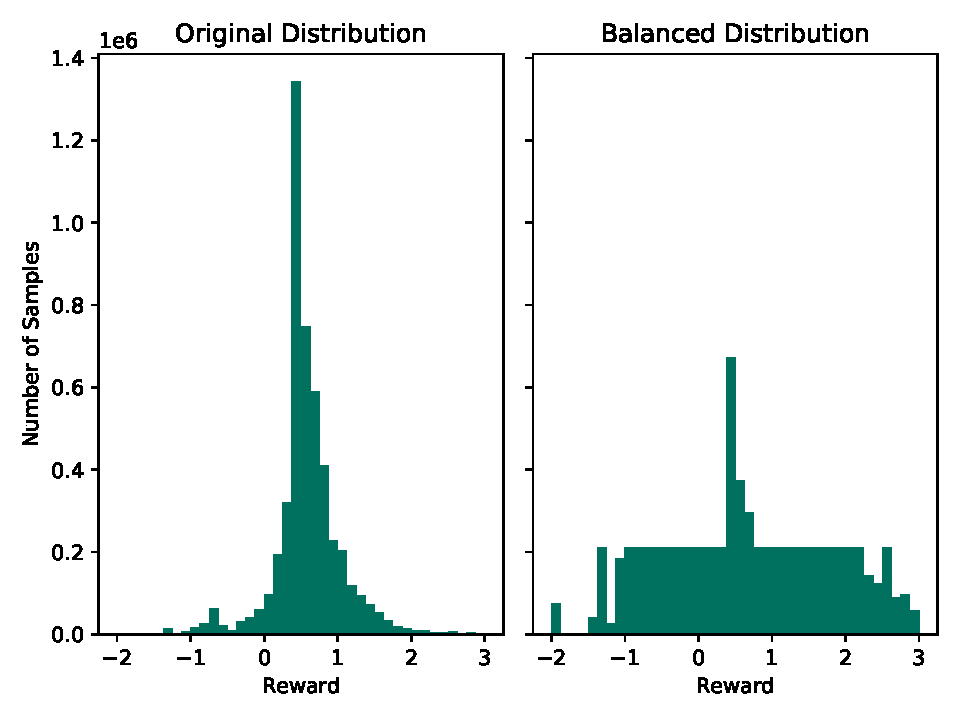
\includegraphics[width=0.75\textwidth]{img/balanced-supervised-dataset-rpi.pdf}
    \caption[Balancing for the AArch64 Dataset]{Balancing for the AArch64 dataset. 
    We duplicate samples with a reward further away from the distribution mean, and delete some samples that are close to the mean.}
    \label{fig:eval:balanced-dataset}
\end{figure}
\Cref{fig:eval:balanced-dataset} illustrates the effect on the distribution of the AArch64-dataset.
The effect for the \aurora dataset is similar.

\subsubsection{Support Vector Regression}
\label{sec:eval:svm}
\acp{svm} have long runtimes when trained with many data points.
We reduced this by randomly selecting 200,000 data points for our model training.

For the AArch64 processor, the average runtime of the instruction schedules generated by this model is between 1.14\% and 1.45\% worse than the runtime of the baseline.
This is the worst result of the parametric models on this processor.

On the \aurora however, we found the best working parametric model to be the \ac{svr} approach combined with clustered instructions.
But it performs still worse than on the AArch64 processor.

Regarding the effects of the dataset balancing and instruction clustering, we see no clear effect.
For the AArch64 processor, the experiments with the balanced datasets perform better.
However, the effect is reversed for the \aurora.
Here, the dataset balancing negatively influenced the performance.

\subsubsection{Neural Network}
\label{sec:eval:nn}
For training the neural network, we use the early stopping scheme.
Once the loss does not improve once for at least $10^{-6}$ in the last 10 epochs, we abort the training.
Therefore, the dataset is split into another training and validation set with a 85/15 split.

The results on the AArch64 processor performs better than the \ac{svr} approach.
With the balanced dataset, we get close to the baseline performance.
However, this approach performs still worse than the baseline.

On the \aurora, the neural network approach performed the worst.
We can also see, that the approach performed the worst with the dataset balancing and the instruction clustering together.


\section{Summary}
The best supervised learning model that we have found is the nearest neighbor approach on the AArch64 processor.
In fact, it is the only one that performed better than the baseline instruction scheduler.
Close to the baseline performance gets the neural network that was trained with the balanced dataset.

For the two dataset variations where we balanced the dataset and clustered similar instructions, we can see that the balancing was helping.
Compare \Cref{tbl:eval:mcts} to see that the models trained with the balanced dataset performed better than with the clustered dataset in three out of four cases.
It even performed better in three out of four cases than the approach with balanced and clustered dataset, and in the one other case it is very close.
So the balancing helped performance wise, and the clustering had a negative influence on the performance.
It seems, that it indeed is important to differenctiate between instructions that only differ in small aspects like the bit width. 

We have seen that our supervised approaches have all worked better on the AArch64 processor.
This was expected due to the smaller dataset and thus the worse average speedup in the \ac{mcts} approach for the \aurora processor.
\Cref{tbl:eval:mcts} shows that the \aurora processor only achieved a 0.30\% speedup in the \ac{mcts} approach.
This value can be seen, as a upper limit for the supervised learning approaches because they are based on the results of the \ac{mcts} approach.

Another important effect, why the approach was not that successful on the \aurora is that it has a out-of-order pipeline.
This means it reschedules the instructions during execution in hardware, so we do not know what is actually executed.
We expected that we would see worse performance on out-of-order hardware.  

Compare speedup with complexity of the problem (number of possible schedulings) vs speedup

Compare CPU Architectures, In-Order vs Out-Of-Order (\url{https://en.wikipedia.org/wiki/Out-of-order_execution})
Here, check speedup vs basic block length, to see if ooo processors perform worse on long basic blocks where it can't see too many instructions ahead

Might be interesting for the discussion: \url{http://www.irisa.fr/alf/downloads/PMA/p241-mcfarlin.pdf}

Mean vs. Median discussion in runtime measurements

\begin{itemize}
    \item Hardware
    \begin{itemize}
        \item Arm Cortex-A53
        \item NEC Aurora
    \end{itemize}
\end{itemize}



Run \ac{mcts} more iterations, because the rest of the schedules still contain many random decision and we can see, that a single decision can make a big difference.

\chapter{Conclusion and Future Work}
\label{sec:conclusion}
In this last chapter, we summarize our work, outline the contributions and results.
Further, we present possible research directions that this thesis opens.

% Answer the research questions
% how good the instruction schedules are that state-of-the-art compilers generate and if we can find better ones
We showed that state-of-the-art compilers do not generate optimal instruction schedules.
With a search approach we are able to find better performing instruction schedules in many cases.
% if it is possible to train a model that can generate better instruction schedules than modern compilers
Further, we showed that it is possible to train a supervised model that is able to generate better instruction schedules than modern compilers.
% investigate the varying influence of the instruction schedules on the performance of in-order and out-of-order processors
In our experiments we have seen that compile-time instruction scheduling has a lower influence on the benchmark runtime on out-of-order processors than on in-order processors.

% Show how you have addressed your aims and objectives
In order to build a methodology that generates optimized instruction schedulers for any novel hardware, we have built our approach on top of the LLVM compiler framework.
We propose an approach that first searches for well performing instruction schedules for a set of of basic block benchmarks.
However, the search takes too much time to do it at compile-time.
Therefore, we build a dataset with the evaluated basic blocks.
To have a fast instruction scheduler, we use this dataset to train a supervised model.

% Explain the significance and implications of your findings
With our approach it is possible to reduce the runtime of compiled computer programs on any hardware.
The influence is especially high for in-order architectures.
Cheaper processors, that are widely used in mobile and edge devices, and also accelerators like \acp{gpu} usually implement in-order architectures.
Shorter runtimes are a good achievement, but with shorter runtimes also comes a reduced energy consumption which is especially important for devices that are powered by batteries.

% Explain the contribution the study makes
Our contribution is a pipeline that automatically optimizes instruction schedulers for any hardware.
Therefore, we developed metrics to select basic blocks with a high influence on the overall runtime of the program.
We extract these basic blocks to execute them in our runtime measurement framework.
The selected and extracted basic blocks are used in an \ac{mcts} approach to find well performing instruction schedules for each basic block.
As a consequence, we get many evaluated scheduling decisions.
We use them to build a datset for training supervised models that can generate well performing instruction schedules for unknwon basic blocks.
Additionally, we made a feasibility study, that showed the potential of optimizing instruction schedulers.

% Explain the limitations of the study
While our work performs well on the in-order architecture, the results are not that good on out-of-order processors.
The search for well performing instruction schedules achieves an average runtime speed up of 0.3\%.
This is an improvement, but it is also an upper limit for the supervised learning models which all perform worse than modern compilers.
Further, we can say that our supervised learning models are still a weakness of our pipeline.
There is definitely potential for improvements and could be a direction for more research.
 
% Lay out questions for further research
Our research layed out multiple directions in which future work could aim.
We used in our search and supervised learning models only basic information, which was mostly just the information about previously schedules instruction and ready-to-schedule instructions.
One type of information that could be useful are heuristics that are already included in the LLVM framework.
This additional information might especially help the supervised learning models.
Common heuristics are for example, if an instruction is part of the critical path of the \ac{dag}, the register pressure, or the distance in the schedule of a candidate instruction to its predecessors.

Further, it would be interesting to extend the supervised learning models with an initialization phase in which the whole \ac{dag} is presented to the instruction scheduler.
It could then extract relevant information from the graph structure of the \ac{dag}.
This would allow the instruction scheduler to plan multiple steps ahead, instead of being limited to the information about previously scheduled instructions and the candidate instructions.
A tool that could help with this are graph neural networks.

Imaginable is also to apply an instruction embedding method to transfer the instructions into a multi-dimensional vector space.
We have discussed some of these approaches in the literature review in \Cref{sec:rw}.
Word embeddings are very succesful in \ac{nlp} tasks and might also help in this task.



% \section{Future Work}

% Nutze mehr Informationen über die Instructions in schedules
% Graph based learning to learn mapping from DAG to schedule
% Learn embeddings word2vec


% What we did is train a heuristic for list scheduling with limited information about the DAG. Our scheduler only learns from ready-to-schedule nodes . It would be interesting to train a graph-nn to analyze the DAG and use it as a single list scheduling heuristic. -> See SAGE Collegeblock Rückseite von Meeting 1.10.
% Include discussion about graph embeddings and put references here
% \cite{mao2019learning}




\listoffigures
\listoftables
\chapter*{List of Acronyms}
% ATTENTION: This file is manipulated by a script. Only add new acronyms and run tools/sort_acronyms.py
\begin{acronym}[LSTM]\itemsep0em
    \acro{ast}[AST]{Abstract Syntax Tree}
    \acro{cpu}[CPU]{central processing unit}
    \acro{dag}[DAG]{Directed Acyclic Graph}
    \acro{io}[I/O]{Input/Output}
    \acro{ir}[IR]{Intermediate Representation}
    \acro{isa}[ISA]{Instruction Set Architecture}
    \acro{lstm}[LSTM]{Long short-term memory}
    \acro{mcts}[MCTS]{Monte Carlo Tree Search}
    \acro{nlp}[NLP]{Natural Language Processing}
    \acro{os}[OS]{Operating System}
    \acro{svm}[SVM]{Support Vector Machine}
    \acro{xfg}[XFG]{Contextual Flow Graph}
\end{acronym}


\printbibliography

\appendix
\chapter{Random Scheduling Experiment}
\label{app:random-scheduling-experiment}
\newcommand{\randomschedulingexperimentplot}[1]{
	\begin{figure}
		\centering
		\includegraphics{img/random-scheduling-experiment/#1.eps}
		\caption{#1}
	\end{figure}
}

\randomschedulingexperimentplot{enc-rc4}
\randomschedulingexperimentplot{espresso}
\randomschedulingexperimentplot{evalloop}
\randomschedulingexperimentplot{fannkuch}
\randomschedulingexperimentplot{fasta}
\randomschedulingexperimentplot{fbench}
\randomschedulingexperimentplot{fdtd-2d}
\randomschedulingexperimentplot{ffbench}
\randomschedulingexperimentplot{fhourstones3.1}
\randomschedulingexperimentplot{fhourstones}
\randomschedulingexperimentplot{five11}
\randomschedulingexperimentplot{fldry}
\randomschedulingexperimentplot{flops-1}
\randomschedulingexperimentplot{flops-2}
\randomschedulingexperimentplot{flops-3}
\randomschedulingexperimentplot{flops}
\randomschedulingexperimentplot{symm}
\randomschedulingexperimentplot{syr2k}
\randomschedulingexperimentplot{syrk}
\randomschedulingexperimentplot{telecomm-CRC32}
\randomschedulingexperimentplot{telecomm-fft}
\randomschedulingexperimentplot{testtrie}
\randomschedulingexperimentplot{treeadd}
\randomschedulingexperimentplot{trisolv}
\randomschedulingexperimentplot{trmm}
\randomschedulingexperimentplot{tsp}
\randomschedulingexperimentplot{uudecode}
\randomschedulingexperimentplot{uuencode}
\randomschedulingexperimentplot{vor}
\randomschedulingexperimentplot{voronoi}
\randomschedulingexperimentplot{whetstone}
\randomschedulingexperimentplot{yacr2}


\end{document}
